%% =============================================================================
%%  Articulo en formato IEEE (clase IEEEtran, modo "journal")
%%  Compilar en Overleaf con pdfLaTeX. Documento principal: main.tex
%%  Bibliografia: referencias.bib (BibTeX, estilo IEEEtran)
%%  Las cifras del texto y las tablas de resultados las genera codigo/gen_tablas_opt.py
%%  (numeros.tex, tabla_*.tex) a partir de resultados/opt/evaluacion_final.json.
%% =============================================================================
\documentclass[journal]{IEEEtran}

% ---- Codificacion e idioma ---------------------------------------------------
\usepackage[utf8]{inputenc}
\usepackage[T1]{fontenc}
\usepackage[spanish,es-tabla,es-nodecimaldot]{babel}
\addto\captionsspanish{\renewcommand{\figurename}{Fig.}\renewcommand{\abstractname}{Abstract}}

% ---- Paquetes ----------------------------------------------------------------
\usepackage{cite}
\usepackage{amsmath,amssymb}
\usepackage{graphicx}
\usepackage{booktabs}
\usepackage[table]{xcolor}
\usepackage{array}
\usepackage{url}

\graphicspath{{figures/}}
% Generado por gen_tablas_opt.py (no editar a mano)
\newcommand{\DelayOfFijo}{13.81}
\newcommand{\DelayOfAct}{10.89}
\newcommand{\DelayOfActAf}{9.63}
\newcommand{\DelayOfActV}{8.34}
\newcommand{\DelayOfMax}{17.44}
\newcommand{\DelayOfPap}{10.95}
\newcommand{\DelayOfPapAf}{9.67}
\newcommand{\DelayOfMdp}{9.35}
\newcommand{\DelayOfFlc}{7.91}
\newcommand{\DelayOfFlcC}{9.97}
\newcommand{\DelayOfMlp}{8.09}
\newcommand{\DelayOfMlpC}{9.46}
\newcommand{\DelayNvFijo}{13.00}
\newcommand{\DelayNvAct}{10.55}
\newcommand{\DelayNvActAf}{9.17}
\newcommand{\DelayNvActV}{7.82}
\newcommand{\DelayNvMax}{16.55}
\newcommand{\DelayNvPap}{10.40}
\newcommand{\DelayNvPapAf}{9.30}
\newcommand{\DelayNvMdp}{8.77}
\newcommand{\DelayNvFlc}{7.40}
\newcommand{\DelayNvFlcC}{9.37}
\newcommand{\DelayNvMlp}{7.53}
\newcommand{\DelayNvMlpC}{8.95}
\newcommand{\DelayVaFijo}{12.29}
\newcommand{\DelayVaAct}{9.23}
\newcommand{\DelayVaActAf}{8.07}
\newcommand{\DelayVaActV}{6.65}
\newcommand{\DelayVaMax}{19.00}
\newcommand{\DelayVaPap}{8.65}
\newcommand{\DelayVaPapAf}{8.06}
\newcommand{\DelayVaMdp}{7.94}
\newcommand{\DelayVaFlc}{6.07}
\newcommand{\DelayVaFlcC}{8.41}
\newcommand{\DelayVaMlp}{6.24}
\newcommand{\DelayVaMlpC}{8.05}
\newcommand{\DelaySaFijo}{40.67}
\newcommand{\DelaySaAct}{54.06}
\newcommand{\DelaySaActAf}{24.13}
\newcommand{\DelaySaActV}{25.61}
\newcommand{\DelaySaMax}{152.25}
\newcommand{\DelaySaPap}{105.87}
\newcommand{\DelaySaPapAf}{58.11}
\newcommand{\DelaySaFlc}{24.29}
\newcommand{\DelaySaFlcC}{25.74}
\newcommand{\DelaySaMlp}{25.10}
\newcommand{\DelaySaMlpC}{24.29}
\newcommand{\RedFijo}{$-$26.1}
\newcommand{\RedAct}{0.6}
\newcommand{\RedActAf}{12.1}
\newcommand{\RedActV}{23.9}
\newcommand{\RedMax}{$-$59.3}
\newcommand{\RedPapAf}{11.7}
\newcommand{\RedMdp}{14.7}
\newcommand{\RedFlc}{27.8}
\newcommand{\RedFlcC}{9.0}
\newcommand{\RedMlp}{26.2}
\newcommand{\RedMlpC}{13.6}
\newcommand{\RedPapOf}{27.8}
\newcommand{\RedActAfOf}{17.8}
\newcommand{\RedActVOf}{5.1}
\newcommand{\RedVistaPapOf}{23.9}
\newcommand{\RedVistaAfOf}{13.4}
\newcommand{\RedPapNv}{28.8}
\newcommand{\RedActAfNv}{19.3}
\newcommand{\RedActVNv}{5.3}
\newcommand{\RedVistaPapNv}{24.8}
\newcommand{\RedVistaAfNv}{14.8}
\newcommand{\RedPapVa}{29.8}
\newcommand{\RedActAfVa}{24.7}
\newcommand{\RedActVVa}{8.7}
\newcommand{\RedVistaPapVa}{23.2}
\newcommand{\RedVistaAfVa}{17.6}
\newcommand{\RedPapSa}{77.1}
\newcommand{\RedActAfSa}{$-$0.7}
\newcommand{\RedActVSa}{5.2}
\newcommand{\RedVistaPapSa}{75.8}
\newcommand{\RedVistaAfSa}{$-$6.2}
\newcommand{\ParMediaPap}{28.2}
\newcommand{\ParMejorPap}{16}
\newcommand{\ParPeorPap}{0}
\newcommand{\ParMinPap}{19.5}
\newcommand{\ParMaxPap}{49.3}
\newcommand{\ParMediaActAf}{22.0}
\newcommand{\ParMejorActAf}{16}
\newcommand{\ParPeorActAf}{0}
\newcommand{\ParMinActAf}{2.9}
\newcommand{\ParMaxActAf}{46.5}
\newcommand{\ParMediaActV}{7.7}
\newcommand{\ParMejorActV}{14}
\newcommand{\ParPeorActV}{0}
\newcommand{\ParMinActV}{0.5}
\newcommand{\ParMaxActV}{26.0}
\newcommand{\ParMediaAct}{31.3}
\newcommand{\ParMejorAct}{16}
\newcommand{\ParPeorAct}{0}
\newcommand{\ParMinAct}{11.4}
\newcommand{\ParMaxAct}{56.8}
\newcommand{\ParMediaFijo}{44.1}
\newcommand{\ParMejorFijo}{16}
\newcommand{\ParPeorFijo}{0}
\newcommand{\ParMinFijo}{39.2}
\newcommand{\ParMaxFijo}{61.2}
\newcommand{\ParMediaMdp}{19.2}
\newcommand{\ParMejorMdp}{16}
\newcommand{\ParPeorMdp}{0}
\newcommand{\ParMinMdp}{2.7}
\newcommand{\ParMaxMdp}{43.5}
\newcommand{\DelayOfFijos}{8.44}
\newcommand{\DelayNvFijos}{7.88}
\newcommand{\DelayVaFijos}{6.56}
\newcommand{\DelaySaFijos}{24.80}
\newcommand{\RedActFijos}{12.3}
\newcommand{\RedPapFijos}{22.9}
\newcommand{\DelayOfReglas}{8.47}
\newcommand{\DelayNvReglas}{7.93}
\newcommand{\DelayVaReglas}{6.55}
\newcommand{\DelaySaReglas}{25.00}
\newcommand{\RedActReglas}{12.0}
\newcommand{\RedPapReglas}{22.6}
\newcommand{\DelayOfGSiete}{8.60}
\newcommand{\DelayNvGSiete}{8.14}
\newcommand{\DelayVaGSiete}{6.85}
\newcommand{\DelaySaGSiete}{25.15}
\newcommand{\RedActGSiete}{10.6}
\newcommand{\RedPapGSiete}{21.4}
\newcommand{\DelayOfGCinco}{8.21}
\newcommand{\DelayNvGCinco}{7.75}
\newcommand{\DelayVaGCinco}{6.41}
\newcommand{\DelaySaGCinco}{25.16}
\newcommand{\RedActGCinco}{14.8}
\newcommand{\RedPapGCinco}{25.1}
\newcommand{\DelayOfGCuatro}{8.04}
\newcommand{\DelayNvGCuatro}{7.58}
\newcommand{\DelayVaGCuatro}{6.20}
\newcommand{\DelaySaGCuatro}{24.38}
\newcommand{\RedActGCuatro}{16.5}
\newcommand{\RedPapGCuatro}{26.6}
\newcommand{\DelayOfSemCero}{8.00}
\newcommand{\DelayNvSemCero}{7.51}
\newcommand{\DelayVaSemCero}{6.21}
\newcommand{\DelaySaSemCero}{24.79}
\newcommand{\RedActSemCero}{16.9}
\newcommand{\RedPapSemCero}{26.9}
\newcommand{\DelayOfSemUno}{8.04}
\newcommand{\DelayNvSemUno}{7.49}
\newcommand{\DelayVaSemUno}{6.24}
\newcommand{\DelaySaSemUno}{24.63}
\newcommand{\RedActSemUno}{16.5}
\newcommand{\RedPapSemUno}{26.6}
\newcommand{\DelayOfSemDos}{7.91}
\newcommand{\DelayNvSemDos}{7.40}
\newcommand{\DelayVaSemDos}{6.07}
\newcommand{\DelaySaSemDos}{24.29}
\newcommand{\RedActSemDos}{17.8}
\newcommand{\RedPapSemDos}{27.8}
\newcommand{\DelayOfLinC}{9.53}
\newcommand{\DelayNvLinC}{8.97}
\newcommand{\DelayVaLinC}{8.10}
\newcommand{\DelaySaLinC}{25.11}
\newcommand{\RedActLinC}{1.0}
\newcommand{\RedPapLinC}{13.0}
\newcommand{\RedActFijo}{$-$43.4}
\newcommand{\RedActAct}{$-$13.1}
\newcommand{\RedActActV}{13.4}
\newcommand{\RedActMax}{$-$81.2}
\newcommand{\RedActPap}{$-$13.8}
\newcommand{\RedActPapAf}{$-$0.4}
\newcommand{\RedActMdp}{2.9}
\newcommand{\RedActFlc}{17.8}
\newcommand{\RedActFlcC}{$-$3.5}
\newcommand{\RedActMlp}{16.0}
\newcommand{\RedActMlpC}{1.7}
\newcommand{\ResDifOf}{0.2}
\newcommand{\ResDifOfMax}{2.1}
\newcommand{\ResDifSa}{4.1}
\newcommand{\ResDifSaMax}{13.9}
\newcommand{\EscNNv}{64}
\newcommand{\EscPapNvRed}{29.7}
\newcommand{\EscPapNvLo}{27.6}
\newcommand{\EscPapNvHi}{31.8}
\newcommand{\EscPapNvP}{$<\!0.001$}
\newcommand{\EscPapNvMejor}{64}
\newcommand{\EscPapNvPeor}{0}
\newcommand{\EscActAfNvRed}{23.3}
\newcommand{\EscActAfNvLo}{20.1}
\newcommand{\EscActAfNvHi}{26.5}
\newcommand{\EscActAfNvP}{$<\!0.001$}
\newcommand{\EscActAfNvMejor}{64}
\newcommand{\EscActAfNvPeor}{0}
\newcommand{\EscActVNvRed}{7.9}
\newcommand{\EscActVNvLo}{6.0}
\newcommand{\EscActVNvHi}{9.8}
\newcommand{\EscActVNvP}{$<\!0.001$}
\newcommand{\EscActVNvMejor}{53}
\newcommand{\EscActVNvPeor}{11}
\newcommand{\EscNVa}{64}
\newcommand{\EscPapVaRed}{30.0}
\newcommand{\EscPapVaLo}{28.3}
\newcommand{\EscPapVaHi}{31.6}
\newcommand{\EscPapVaP}{$<\!0.001$}
\newcommand{\EscPapVaMejor}{64}
\newcommand{\EscPapVaPeor}{0}
\newcommand{\EscActAfVaRed}{27.1}
\newcommand{\EscActAfVaLo}{24.8}
\newcommand{\EscActAfVaHi}{29.3}
\newcommand{\EscActAfVaP}{$<\!0.001$}
\newcommand{\EscActAfVaMejor}{64}
\newcommand{\EscActAfVaPeor}{0}
\newcommand{\EscActVVaRed}{10.1}
\newcommand{\EscActVVaLo}{8.8}
\newcommand{\EscActVVaHi}{11.5}
\newcommand{\EscActVVaP}{$<\!0.001$}
\newcommand{\EscActVVaMejor}{64}
\newcommand{\EscActVVaPeor}{0}
\newcommand{\EscNSa}{32}
\newcommand{\EscPapSaRed}{69.5}
\newcommand{\EscPapSaLo}{64.3}
\newcommand{\EscPapSaHi}{74.7}
\newcommand{\EscPapSaP}{$<\!0.001$}
\newcommand{\EscPapSaMejor}{32}
\newcommand{\EscPapSaPeor}{0}
\newcommand{\EscActAfSaRed}{$-$0.3}
\newcommand{\EscActAfSaLo}{$-$1.3}
\newcommand{\EscActAfSaHi}{0.6}
\newcommand{\EscActAfSaP}{0.36}
\newcommand{\EscActAfSaMejor}{14}
\newcommand{\EscActAfSaPeor}{18}
\newcommand{\EscActVSaRed}{4.4}
\newcommand{\EscActVSaLo}{3.0}
\newcommand{\EscActVSaHi}{5.9}
\newcommand{\EscActVSaP}{$<\!0.001$}
\newcommand{\EscActVSaMejor}{30}
\newcommand{\EscActVSaPeor}{2}
\newcommand{\MedOfFijos}{8.47}
\newcommand{\SdOfFijos}{0.04}
\newcommand{\MedNvFijos}{7.89}
\newcommand{\SdNvFijos}{0.03}
\newcommand{\MedVaFijos}{6.56}
\newcommand{\SdVaFijos}{0.02}
\newcommand{\MedSaFijos}{24.94}
\newcommand{\SdSaFijos}{0.13}
\newcommand{\NSemFijos}{3}
\newcommand{\RedPapMedFijos}{22.7}
\newcommand{\RedActAfMedFijos}{12.0}
\newcommand{\RedActVMedFijos}{$-$1.6}
\newcommand{\MedOfReglas}{8.44}
\newcommand{\SdOfReglas}{0.03}
\newcommand{\MedNvReglas}{7.87}
\newcommand{\SdNvReglas}{0.05}
\newcommand{\MedVaReglas}{6.55}
\newcommand{\SdVaReglas}{0.00}
\newcommand{\MedSaReglas}{24.90}
\newcommand{\SdSaReglas}{0.11}
\newcommand{\NSemReglas}{3}
\newcommand{\RedPapMedReglas}{23.0}
\newcommand{\RedActAfMedReglas}{12.4}
\newcommand{\RedActVMedReglas}{$-$1.2}
\newcommand{\MedOfGSiete}{8.55}
\newcommand{\SdOfGSiete}{0.05}
\newcommand{\MedNvGSiete}{8.11}
\newcommand{\SdNvGSiete}{0.04}
\newcommand{\MedVaGSiete}{6.84}
\newcommand{\SdVaGSiete}{0.02}
\newcommand{\MedSaGSiete}{24.70}
\newcommand{\SdSaGSiete}{0.40}
\newcommand{\NSemGSiete}{3}
\newcommand{\RedPapMedGSiete}{21.9}
\newcommand{\RedActAfMedGSiete}{11.2}
\newcommand{\RedActVMedGSiete}{$-$2.5}
\newcommand{\MedOfGCinco}{8.19}
\newcommand{\SdOfGCinco}{0.05}
\newcommand{\MedNvGCinco}{7.72}
\newcommand{\SdNvGCinco}{0.08}
\newcommand{\MedVaGCinco}{6.44}
\newcommand{\SdVaGCinco}{0.09}
\newcommand{\MedSaGCinco}{25.15}
\newcommand{\SdSaGCinco}{0.09}
\newcommand{\NSemGCinco}{3}
\newcommand{\RedPapMedGCinco}{25.2}
\newcommand{\RedActAfMedGCinco}{14.9}
\newcommand{\RedActVMedGCinco}{1.7}
\newcommand{\MedOfGCuatro}{8.05}
\newcommand{\SdOfGCuatro}{0.02}
\newcommand{\MedNvGCuatro}{7.56}
\newcommand{\SdNvGCuatro}{0.01}
\newcommand{\MedVaGCuatro}{6.20}
\newcommand{\SdVaGCuatro}{0.04}
\newcommand{\MedSaGCuatro}{24.50}
\newcommand{\SdSaGCuatro}{0.11}
\newcommand{\NSemGCuatro}{3}
\newcommand{\RedPapMedGCuatro}{26.5}
\newcommand{\RedActAfMedGCuatro}{16.4}
\newcommand{\RedActVMedGCuatro}{3.4}
\newcommand{\MedOfGTres}{7.98}
\newcommand{\SdOfGTres}{0.06}
\newcommand{\MedNvGTres}{7.47}
\newcommand{\SdNvGTres}{0.06}
\newcommand{\MedVaGTres}{6.18}
\newcommand{\SdVaGTres}{0.09}
\newcommand{\MedSaGTres}{24.57}
\newcommand{\SdSaGTres}{0.25}
\newcommand{\NSemGTres}{3}
\newcommand{\RedPapMedGTres}{27.1}
\newcommand{\RedActAfMedGTres}{17.1}
\newcommand{\RedActVMedGTres}{4.2}
\newcommand{\PdMaxDif}{0.7}
                          % cifras generadas desde los resultados

\newcommand{\fuente}[1]{\par\vspace{3pt}\noindent{\scriptsize\textit{Fuente:} #1\par}}
\renewcommand{\thetable}{\arabic{table}}
\newcommand{\qbar}{\bar{q}}              % tasa media de llegada (veh/s)
\newcommand{\FLC}{FLC-O}
\newcommand{\PMR}{Pappis y Mamdani reconstruido}

% =============================================================================
\begin{document}

\title{Mejora de un controlador de semáforos de lógica difusa para una intersección aislada: optimización del controlador de Pappis y Mamdani (1977)}

\author{Raul Nolberto Quispe Saya and Kevin Luis Valero Ccacya%
\thanks{R. N. Quispe Saya y K. L. Valero Ccacya pertenecen a la Escuela Profesional de Ingeniería Electrónica, Universidad Nacional de San Agustín de Arequipa, Arequipa, Perú (correos electrónicos: rquispesa@unsa.edu.pe, kvaleroc@unsa.edu.pe).}}

\markboth{Quispe Saya y Valero Ccacya: Mejora de un controlador difuso de semáforos}%
{Quispe Saya y Valero Ccacya: Mejora de un controlador difuso de semáforos}

\maketitle

% =============================================================================
\begin{abstract}
This paper improves the 1977 Pappis--Mamdani fuzzy-logic traffic-signal controller for an isolated two-phase intersection by optimization, taking the authors' earlier reconstruction of that controller as the baseline (the printed rules, sets and operators, with the inputs $A$ and $Q$ defined here; it reproduces the printed Table VIII with a mean error of 9.2\,\%). First, the delay is measured as the sum of the queues over the whole horizon, which extends the original's per-cycle definition and also counts the vehicles still queued at the end. Second, a vectorized simulator is built that reproduces the reference simulator exactly (zero difference in six controllers) and runs about twenty times faster. Third, the optimal policy for known flows without look-ahead is computed by dynamic programming and used as a benchmark. Fourth, a 27-rule fuzzy controller (FLC-O) with singleton consequents is trained with CMA-ES; its membership functions, rules and look-ahead weights (42 parameters) are learned on random flows that are not those used for evaluation. On the 16 flow pairs of the original Table VIII, with 20 replications of 7200 s, FLC-O reduces the mean delay from \DelayOfPap{} to \DelayOfFlc{} s/veh (\RedFlc\,\%) with respect to the reconstructed controller, which has the same 10-s look-ahead of arrivals, is significantly better in \ParMejorPap{} of 16 pairs and never significantly worse. It also improves a tuned actuated controller by \RedActAfOf\,\%, but that controller has no look-ahead: given the same 10-s look-ahead, the tuned actuated controller gains \RedVistaAfOf\,\% on its own and the remaining gain of FLC-O is \RedActVOf\,\% (significantly better in \ParMejorActV{} of 16 pairs, never worse). The gains hold on unseen flows and with time-varying demand. Without look-ahead, the best learned controller improves the tuned actuated one by only \RedActMlpC\,\%. Near saturation (3000 to 3300 veh/h) FLC-O is on par with the tuned actuated controller (\DelaySaFlc{} against \DelaySaActAf{} s/veh; no significant difference, $p=\EscActAfSaP$) and far better than the reconstructed one (\DelaySaPap{}). The contribution is empirical (optimization and benchmarking), not a new control theory. As in the 1977 study, all results come from computer simulation of the intersection model; no hardware was built or installed and no field data were used.
\end{abstract}

\begin{IEEEkeywords}
Fuzzy logic control, Mamdani inference, CMA-ES, dynamic programming, traffic signal control, vehicle delay, simulation.
\end{IEEEkeywords}

\IEEEpeerreviewmaketitle

\noindent{\footnotesize\textbf{\textit{Resumen}---}Este artículo mejora, mediante optimización, el controlador de semáforos con lógica difusa de Pappis y Mamdani (1977) para una intersección aislada de dos fases, y toma como punto de partida la reconstrucción de ese controlador hecha antes por los autores (las reglas, los conjuntos y los operadores impresos, con las entradas $A$ y $Q$ definidas aquí; reproduce la Tabla~VIII impresa con un error medio de 9.2\,\%). Primero se mide el retardo como la suma de las colas durante todo el horizonte, que extiende la definición por ciclo del original y cuenta también a los vehículos que siguen en cola al final. Segundo, se construye un simulador vectorizado que reproduce exactamente al simulador de referencia (diferencia nula en seis controladores) y es unas veinte veces más rápido. Tercero, se calcula por programación dinámica la política óptima para caudales conocidos y sin vista adelante, que se usa como cota. Cuarto, se entrena con CMA-ES un controlador difuso de 27 reglas con consecuentes numéricos (FLC-O) cuyas funciones de pertenencia, reglas y pesos de la vista adelante (42 parámetros) se aprenden con caudales sorteados que no son los de la evaluación. En los 16 pares de caudales de la Tabla~VIII del original, con 20 réplicas de 7200\,s, FLC-O reduce el retardo medio de \DelayOfPap{} a \DelayOfFlc{}\,s/veh (\RedFlc\,\%) respecto del controlador reconstruido, que tiene la misma vista adelante de 10\,s, es significativamente mejor en \ParMejorPap{} de 16 pares y nunca significativamente peor. También mejora en \RedActAfOf\,\% a un actuado afinado, pero ese controlador no tiene vista adelante: con la misma vista adelante de 10\,s, el actuado afinado gana \RedVistaAfOf\,\% por sí solo y la ganancia que queda a FLC-O es de \RedActVOf\,\% (significativamente mejor en \ParMejorActV{} de 16 pares, nunca peor). Las ganancias se mantienen con caudales no vistos y con demanda variable. Sin vista adelante, el mejor controlador aprendido mejora al actuado afinado solo en \RedActMlpC\,\%. Cerca de la saturación (de 3000 a 3300\,veh/h), FLC-O queda a la par del actuado afinado (\DelaySaFlc{} frente a \DelaySaActAf{}\,s/veh; sin diferencia significativa, $p=\EscActAfSaP$) y muy por debajo del controlador reconstruido (\DelaySaPap{}). La contribución es empírica (optimización y comparación), no una nueva teoría de control. Como en el estudio de 1977, todos los resultados salen de la simulación en computadora del modelo de la intersección; no se construyó ni se instaló hardware y no se usaron datos de campo.\par}
\vspace{2pt}
\noindent{\footnotesize\textbf{\textit{Palabras clave}---}Control con lógica difusa, inferencia de Mamdani, CMA-ES, programación dinámica, control de semáforos, retardo vehicular, simulación.\par}

% =============================================================================
\section{Introducción}
\label{sec:intro}

\IEEEPARstart{E}{l} control de las señales luminosas de una intersección es uno de los problemas más estudiados de la ingeniería de tránsito. En la intersección aislada consiste en repartir el tiempo de verde entre las fases para reducir una medida de desempeño; la más habitual es el retardo medio por vehículo \cite{Pappis1977,Papageorgiou2003}. Los métodos clásicos fijan el ciclo y los verdes con los caudales medios \cite{Webster1958,Webster1966,Miller1963,Allsop1971}, los controladores actuados y adaptativos los modifican con detectores \cite{Hunt1982,Lowrie1982,Mirchandani2001}, y una tercera familia traduce el criterio de un operador a reglas lingüísticas ejecutadas con lógica difusa \cite{Zadeh1965,Zadeh1973,MamdaniAssilian1975}. Su referencia fundacional en tráfico es Pappis y Mamdani \cite{Pappis1977}: dos calles unidireccionales sin giros, un controlador que interviene a los 7, 17, 27, 37 y 47\,s del verde efectivo y decide con 25 reglas cuántos segundos extenderlo (de 1 a 10\,s) o si cambia de fase.

Un trabajo previo de los autores replicó ese controlador a partir de la publicación original, con una única fuente, y lo validó elemento por elemento (conjuntos, operadores, reglas y ejemplo trabajado) y con 20 réplicas estadísticas. La réplica dejó tres hechos. Primero, el controlador mejora al ciclo fijo de Webster en 16 de 16 combinaciones de caudal, como publicó el original. Segundo, la línea base de la Tabla~VIII del original se llama «vehicle-actuated», pero sus retardos son los del ciclo fijo óptimo de su Tabla~I, que el original supone equivalentes a los de un actuado eficiente (p.~709); frente a un actuado por detector simulado, el controlador no es mejor en promedio. Tercero, el original obtuvo sus reglas por prueba y error y habla de «satisficing control» (p.~714), es decir, de un conjunto suficientemente bueno y no necesariamente el mejor. Este trabajo pregunta cuánto puede mejorarse ese controlador si se optimizan sus parámetros y su estructura con un procedimiento reproducible, y contra qué referencias justas hay que medirlo.

Las contribuciones son:
\begin{enumerate}
\item Una medida del retardo que cuenta toda la espera hasta el horizonte y un simulador vectorizado que da, escenario por escenario, exactamente los mismos retardos que el de referencia y es unas veinte veces más rápido, lo que hace posible optimizar.
\item Una cota de lo alcanzable sin ver el futuro: la política óptima por programación dinámica para caudales conocidos, validada contra la simulación.
\item \FLC{}: un controlador difuso de 27 reglas, con consecuentes numéricos, que decide cada segundo y cuyos 42 parámetros se entrenan con CMA-ES; las reglas siguen siendo legibles.
\item Un protocolo sin fuga de información: entrenamiento con caudales sorteados, y prueba en los 16 pares de la Tabla~VIII del original y en conjuntos adicionales (caudales no vistos, demanda variable, cerca de la saturación), con estadística pareada.
\item Un análisis de qué información y qué diseño producen la mejora: vista adelante frente a causal, verde mínimo, número de reglas y comparación con una política neuronal.
\end{enumerate}

La contribución es empírica: se optimiza y se compara con un protocolo reproducible un controlador que integra elementos conocidos (inferencia difusa con consecuentes numéricos, particiones de Ruspini, CMA-ES); no es una nueva teoría de control.

\textbf{Alcance: un estudio de simulación.} Todo el trabajo es computacional: los controladores se programan y se evalúan en un modelo de simulación de la intersección. No se construyó ni se instaló hardware (detectores, controladores de semáforo, PLC o microcontroladores), no se compraron equipos y no se usaron datos de campo. Es el mismo alcance del original, cuyos resultados también salen de corridas de 7200\,s simuladas en computadora (pp.~709 y~714). Ese alcance es el que permite comparar con su Tabla~VIII bajo el mismo modelo, con las mismas llegadas para todos los controladores y con 20 réplicas, algo imposible en una intersección real, donde el tráfico no se repite. Las conclusiones valen dentro de ese modelo; llevar \FLC{} a una intersección real exigiría detectores aguas arriba para la vista adelante, verificar el verde mínimo con la norma local y validarlo con tráfico real, lo que queda como trabajo futuro (Sec.~\ref{sec:discusion}). Por eso el único equipo que se reporta es la computadora en que se ejecutaron las simulaciones (Sección «Disponibilidad del código»).

La Sección~\ref{sec:sota} revisa el estado del arte; la \ref{sec:modelo}, el modelo y la medida del retardo; la \ref{sec:pappis}, el controlador de Pappis y Mamdani; la \ref{sec:simulador}, el simulador vectorizado y la cota óptima; la \ref{sec:opt}, los controladores optimizados; la \ref{sec:protocolo}, el protocolo experimental; la \ref{sec:resultados}, los resultados; la \ref{sec:discusion} los discute y la \ref{sec:conclusiones} concluye.

% =============================================================================
\section{Estado del arte}
\label{sec:sota}

\subsection{Control de una intersección aislada}
El \emph{control de tiempo fijo} repite un plan calculado con los caudales medios; Webster \cite{Webster1958} dedujo el ciclo que minimiza el retardo, y Webster y Cobbe \cite{Webster1966}, Miller \cite{Miller1963}, Allsop \cite{Allsop1971} y TRANSYT \cite{Robertson1969} estudiaron sus ajustes. Su limitación es que los retardos reales exceden los óptimos cuando los caudales se apartan de los de diseño \cite{Pappis1977}. Un \emph{controlador actuado} prolonga el verde mientras los detectores ven llegadas, entre un mínimo y un máximo; los \emph{sistemas adaptativos} optimizan parámetros en línea: SCOOT \cite{Hunt1982}, SCATS \cite{Lowrie1982} y RHODES \cite{Mirchandani2001}; Papageorgiou \emph{et al.} \cite{Papageorgiou2003} revisan las estrategias urbanas. Un controlador de \emph{presión máxima} da paso al brazo con mayor presión y tiene garantías de estabilidad en redes \cite{Varaiya2013}. En todos ellos el desempeño estándar es el retardo medio por vehículo.

\subsection{Lógica difusa y control de semáforos}
Zadeh \cite{Zadeh1965,Zadeh1973,Zadeh1975} introdujo los conjuntos difusos, el enfoque lingüístico y la variable lingüística; Mamdani y Assilian \cite{MamdaniAssilian1975} los aplicaron al control de una planta, con el «y» como mínimo y el «si no» como máximo. Variantes posteriores son los consecuentes funcionales de Takagi y Sugeno \cite{TakagiSugeno1985} y la red adaptativa de Jang \cite{Jang1993}. En semáforos, Pappis y Mamdani \cite{Pappis1977} afinaron las reglas por prueba y error. Después, Trabia \emph{et al.} \cite{Trabia1999} proponen un controlador de dos etapas con detectores de lazo; Niittymäki y Pursula \cite{Niittymaki2000} desarrollan principios y algoritmos y citan una comparación de 1996 entre el algoritmo de Pappis y Mamdani y el principio de extensión \cite{Pursula1996}; Bingham \cite{Bingham2001} ajusta las funciones de pertenencia con una red neuronal y aprendizaje por refuerzo; y Murat y Gedizlioglu \cite{Murat2005} presentan FLMuSiC. Entre 2021 y 2026 siguen Ali \emph{et al.} \cite{Ali2021} (difuso con la fórmula de Webster en SUMO), Jiang \emph{et al.} \cite{Jiang2021} (esquema de dos etapas), Vuong \emph{et al.} \cite{Vuong2021} (ANFIS) y Shaheen \emph{et al.} \cite{Shaheen2026} (variantes intuicionista y de tipo 2). Estas obras conservan la estructura lingüística de Pappis y Mamdani pero ninguna optimiza, con un protocolo de prueba separado, el controlador original frente a un actuado afinado y una cota óptima.

\subsection{Aprendizaje por refuerzo y optimización de políticas}
Una línea paralela formula el control como decisión secuencial: Abdulhai \emph{et al.} \cite{Abdulhai2003} aplican \emph{Q-learning} a una intersección aislada y el aprendizaje profundo \cite{Mnih2015,Genders2016,Wei2018,Chu2020} se evalúa en simuladores y con datos reales; Noaeen \emph{et al.} \cite{Noaeen2022} y Michailidis \emph{et al.} \cite{Michailidis2025} lo revisan, y Vlasceanu \emph{et al.} \cite{Vlasceanu2025} contrastan un difuso con \emph{Q-learning}. Estos métodos aprenden la política de los datos pero dependen de la definición de estado y recompensa y de hiperparámetros cuya documentación incompleta dificulta comparar \cite{Henderson2018}. Aquí se usa una estrategia evolutiva, CMA-ES \cite{Hansen2001,Hansen2016}, para entrenar los parámetros de un controlador difuso y de una política neuronal: es una optimización de caja negra del retardo medio simulado, sin gradiente, adecuada para pocos parámetros y objetivos con escalones como el de decidir cuándo cortar el verde.

\subsection{Brecha}
Falta, en las fuentes consultadas, una comparación en la que el controlador difuso de 1977, su versión afinada y un difuso nuevo se midan con un mismo protocolo contra un actuado también afinado, una cota óptima y una política aprendida, separando entrenamiento, validación y prueba, y reportando cuánto de la mejora depende de ver el futuro cercano.

% =============================================================================
\section{Modelo de la intersección y medida del retardo}
\label{sec:modelo}

El modelo es el del original \cite{Pappis1977}, con las precisiones que se indican. \emph{Del original} (pp.~708--709): dos brazos unidireccionales sin giros que comparten un cruce, flujo de saturación de 3600\,veh/h ($s=1$\,veh/s), un tiempo perdido total de 10\,s por ciclo y llegadas aleatorias que se deciden cada segundo comparando un número pseudoaleatorio con la tasa media de llegada, de modo que llega a lo sumo un vehículo por segundo y brazo, $\alpha_n=1$ con probabilidad $\qbar_i$ (llegadas de Bernoulli); cada simulación dura 7200\,s. \emph{Definido aquí}, porque el original no lo precisa: el tiempo avanza en pasos de 1\,s, los 10\,s por ciclo se reparten en $5$\,s en cada cambio de fase, durante el rojo nadie sale, durante el verde salen $s$ vehículos por segundo mientras haya cola, y un vehículo que llega con la cola vacía cruza sin esperar. Si $Q_{i,n}$ es la cola del brazo $i$ al final del segundo $n$, la espera total de todos los vehículos hasta el horizonte $H$ y el retardo medio por vehículo son
\begin{equation}
D=\sum_{n=0}^{H-1}\bigl(Q_{1,n}+Q_{2,n}\bigr),\qquad d_m=\frac{D}{\sum_{n<H}(\alpha_{1,n}+\alpha_{2,n})}.
\label{eq:dm}
\end{equation}
La primera igualdad es una deducción, no una convención: el retardo de un vehículo es el número de finales de segundo en que está en cola (de su llegada a su salida, o al horizonte si sigue en cola), y sumar primero por vehículo y luego por segundo, o al revés, da la suma de las colas, es decir, el área bajo las curvas de cola; la segunda es la definición de media. Es la definición del original, que calcula la espera de cada ciclo sumando, segundo a segundo, los vehículos en cola durante el rojo y el verde (p.~708), aplicada a todo el horizonte. El original no dice qué hacer con los vehículos que siguen en cola al terminar la simulación. La réplica anterior de los autores solo sumaba la espera de los vehículos que ya habían salido: los que seguían en cola contaban en el denominador y aportaban cero, lo que subestima el retardo, en especial con colas largas. En este artículo el retardo es siempre \eqref{eq:dm}, que incluye la espera residual. Para el controlador de Pappis y Mamdani, la diferencia entre ambas convenciones es de \ResDifOf\,\% en promedio en el conjunto oficial (hasta \ResDifOfMax\,\% en un escenario) y de \ResDifSa\,\% en promedio cerca de la saturación (hasta \ResDifSaMax\,\%).

\begin{table*}[!t]
\centering
\caption{Notación (cada símbolo con un único significado)}
\label{tab:notacion}
\scriptsize
\setlength{\tabcolsep}{3pt}
\begin{tabular}{@{}cp{0.31\textwidth}cp{0.31\textwidth}@{}}
\toprule
Símbolo & Significado & Símbolo & Significado \\
\midrule
$\alpha_{i,n}$ & llegada al brazo $i$ en el segundo $n$ (0 o 1) & $\qbar_i$ & tasa de llegada (veh/s) \\
$Q_{i,n}$ & cola del brazo $i$ al final del segundo $n$ & $d_m$, $D$ & retardo medio (s/veh) y total (veh$\cdot$s) \\
$H$, $n_e$ & horizonte (s) y número de escenarios & $s$, $L$ & flujo de saturación y tiempo perdido por ciclo \\
$y_i$, $Y$, $C_0$, $g_i$ & razón de flujo, su suma, ciclo y verde de Webster & $T,E,A,Q$ & variables de Pappis y Mamdani (tiempo, extensión, arribos, cola) \\
$\gamma(e)$, $e^*$ & grado y extensión elegida ($0$: cambiar) & $Q_g$, $Q_r$ & colas del brazo con verde y del brazo en rojo \\
$G$, $R$, $V$ & demanda en verde, presión en rojo, verde transcurrido (\FLC{}) & $W_g(l)$, $W_r(l)$ & llegadas previstas en los $l$ s siguientes \\
$c_{ijk}$, $w_{ijk}$, $u$ & consecuente, fuerza de la regla y salida de \FLC{} & $\omega_k,\rho_k$ & pesos de la vista adelante \\
$g_{\min}$, $g_{\max}$ & verde mínimo y máximo & $J(\theta)$ & objetivo de entrenamiento \\
$a_e$, $q_e$ & entradas $A$ y $Q$ de Pappis y Mamdani para una extensión de $e$ s & $Q_V$ & vehículos llegados al brazo en rojo desde que empezó el verde (lectura de $q_e$) \\
$k_1,k_2,k_3$ & nudos de los conjuntos de $G$, $R$ o $V$ & $\mu_{\text{bajo}},\mu_{\text{medio}},\mu_{\text{alto}}$ & pertenencias de \FLC{} \\
\bottomrule
\end{tabular}
\fuente{elaboración propia; los símbolos de Pappis y Mamdani \cite{Pappis1977} se conservan, salvo la tasa de llegada, que se escribe $\qbar_i$ para reservar $q$ a las colas.}
\end{table*}

La línea base clásica es el ciclo fijo de Webster, con $y_i=\qbar_i/s$, $Y=y_1+y_2$, $L=10$\,s:
\begin{equation}
C_0=\frac{1.5\,L+5}{1-Y},\qquad g_i=\frac{y_i}{Y}\,(C_0-L),
\label{eq:webster}
\end{equation}
tomados de Webster \cite{Webster1958} tal como los imprime el original (p.~709), con los verdes redondeados al segundo más próximo. El reparto $g_i\propto y_i$ se deduce de igualar los grados de saturación de las dos fases, $X_i=y_iC/g_i$, con $g_1+g_2=C-L$; las constantes $1.5$ y $5$ del ciclo son un ajuste empírico de Webster y no se deducen. El ciclo fijo necesita conocer los caudales; los controladores de las secciones siguientes no los conocen.

% =============================================================================
\section{El controlador de Pappis y Mamdani}
\label{sec:pappis}

\subsection{Estructura}
\label{sec:estructura}
El controlador interviene a los 7, 17, 27, 37 y 47\,s del verde y decide la extensión $e^*\in\{0,1,\dots,10\}$ s del verde; $e^*=0$ cambia de fase y el verde máximo es de 57\,s. Usa cuatro variables sobre universos discretos: el tiempo $T$ y la extensión $E$ ($1$ a $10$\,s), los arribos $A$ ($1$ a $10$ veh en el brazo con paso) y la cola $Q$ ($4$ a $32$ veh en el brazo en rojo). Las reglas usan versiones monótonas de los conjuntos con dos operadores: si $x_0$ es el punto donde $\mu_A$ es máxima,
\begin{equation}
\begin{aligned}
\mu_{lt(A)}(x)&=\begin{cases}1-\mu_A(x), & x<x_0\\ 0, & x\ge x_0\end{cases}\\
\mu_{mt(A)}(x)&=\begin{cases}0, & x<x_0\\ 1-\mu_A(x), & x\ge x_0\end{cases}
\end{aligned}
\label{eq:mtlt}
\end{equation}
de modo que $lt(A)\cup mt(A)=\overline{A}$ y $lt(A)\cap mt(A)=\emptyset$ en todo el universo, incluido $x_0$, porque en cada $x$ solo una de las dos es no nula; \eqref{eq:mtlt} son las definiciones del original (p.~710). Las 25 reglas son «si $T=t$ y $A=mt(a)$ y $Q=lt(q)$ entonces $E=e$», con $E=T$, cinco por intervención. La contribución de la regla $j$ a la extensión $e$ es $\min\{\mu_{T_j}(e),\mu_{mt(A_j)}(a_e),\mu_{lt(Q_j)}(q_e),\mu_{E_j}(e)\}$, el grado es $\gamma(e)=\max_j$ de ellas, y la decisión es
\begin{equation}
e^*=\begin{cases}\max\{e:\gamma(e)=\gamma_{\max}\}, & \gamma_{\max}\ge 0.5\\ 0, & \gamma_{\max}<0.5\end{cases}
\label{eq:decision}
\end{equation}
La ecuación \eqref{eq:decision} reúne tres enunciados del original: se elige la extensión de mayor grado (p.~713), si todos son menores que 0.5 la fase cambia (p.~714) y, en un empate, se toma la mayor extensión (p.~714). La Fig.~\ref{fig:fuzzificacion} muestra los conjuntos con los valores impresos en el original.

\begin{figure*}[!t]
\centering
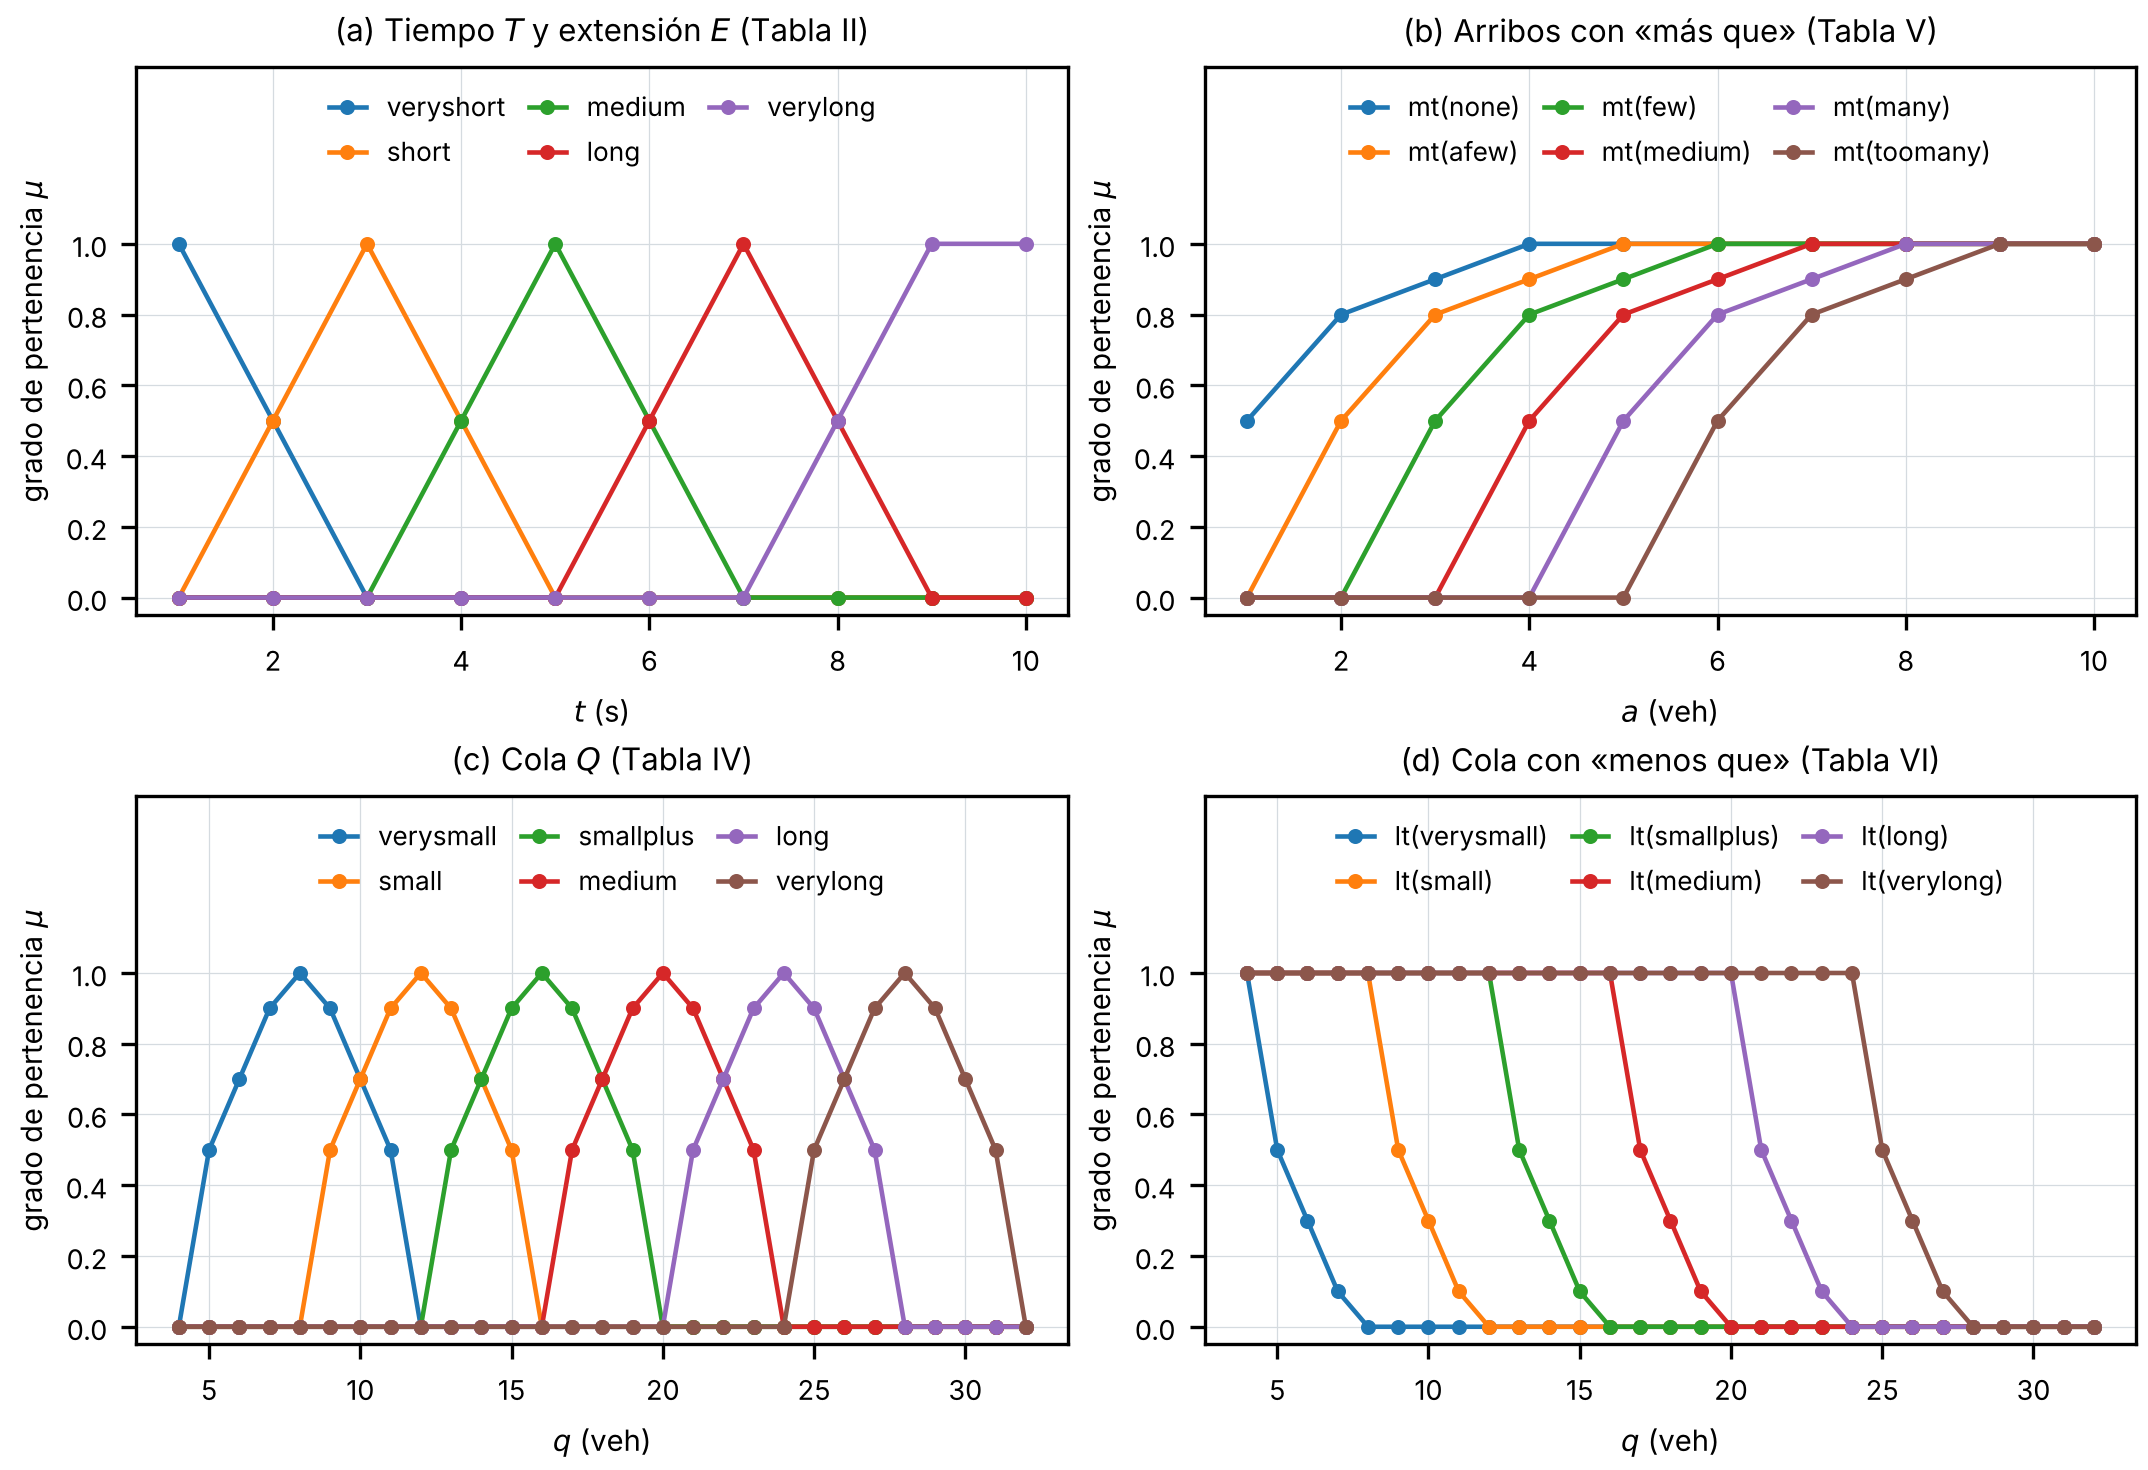
\includegraphics[width=\textwidth]{fig_fuzzificacion_ieee.png}
\caption{Curvas de fuzzificación del controlador de Pappis y Mamdani: (a) tiempo y extensión; (b) arribos con el operador «más que»; (c) colas; (d) colas con el operador «menos que». Trazadas con los valores impresos en el artículo original.}
\label{fig:fuzzificacion}
\end{figure*}

\subsection{Definición de las entradas $A$ y $Q$}
\label{sec:lecturas}
\textbf{Qué dice el original.} Los detectores, instalados lejos de la línea de parada, informan en cada intervención de las llegadas a ambos brazos en los segundos siguientes (p.~709). $A$ es el número de vehículos que llegan al brazo con paso y $Q$ la cola (p.~710). En su ejemplo (p.~713) las llegadas de cada segundo se acumulan en $\beta_e$, los vehículos que cruzan el punto crítico en los $e$ segundos siguientes, y $\beta'_e=Q+\sum_{i\le e}x'_i$, la cola actual del brazo en rojo más las llegadas a él; la entrada $(t_i,a_j,q_k,e_l)$ de la matriz del algoritmo usa $t=e$, $a=\beta_e$ y $q=\beta'_e$.

\textbf{Qué no queda determinado.} El ejemplo ilustra el cálculo con vectores dados: no fija si, en una simulación, $Q$ es la cola total o solo los vehículos llegados desde que empezó el verde, ni cómo cuentan en $A$ los que ya esperan en el brazo con paso. Aplicadas al pie de la letra a este modelo (arribos acumulados y cola total evaluada en $\beta'_e$), las definiciones hacen que el controlador corte el verde en torno a los 9\,s en cuanto sube el caudal y el sistema se sature (error medio de 641\,\% frente a los retardos impresos; Tabla~S2).

\textbf{Qué se define aquí.} Es una decisión de diseño de este trabajo, no una afirmación sobre cómo lo programaron Pappis y Mamdani: $a_e=\min(e,\,Q_g+\sum_{i\le e}x_i)$, con $Q_g$ la cola del brazo con paso y $x_i$ las llegadas previstas en el segundo $i$, es decir, los vehículos que cruzan en los $e$ segundos siguientes, limitados por 1\,veh/s e incluyendo la cola del verde; y $q_e=Q_V$, los vehículos llegados al brazo en rojo desde que empezó el verde actual, sin la cola que ya tenía al empezar. Esta última es la diferencia con el ejemplo del original. Se eligió entre las ocho combinaciones razonables (Tabla~S2) porque es la única que reproduce el comportamiento publicado: con 20 réplicas de 7200\,s y números aleatorios comunes, el controlador mejora al ciclo fijo en 16 de 16 combinaciones de caudal, con un error medio de 9.2\,\% frente a los retardos impresos de la Tabla~VIII (máximo 18.6\,\%), y el modelo reproduce la tabla de validación del original con un error medio de 2.1\,\%. Todo lo que sigue usa esta definición para el controlador «Pappis y Mamdani».

Una propiedad del modelo importa para lo que sigue: las llegadas de los próximos 10\,s ($x_i$, $x'_i$) se suponen conocidas, como si detectores aguas arriba midieran los vehículos en tránsito (pp.~709 y 713). Es la \emph{vista adelante}. El controlador de la Sección~\ref{sec:opt} la conserva, y la Sección~\ref{sec:resultados} mide cuánto de su mejora depende de ella.

% =============================================================================
\section{Simulador vectorizado y cota óptima}
\label{sec:simulador}

\subsection{Simulador vectorizado}
\label{sec:vectorizado}
Optimizar exige evaluar un controlador en cientos de escenarios miles de veces. Se reescribió el simulador para simular $n_e$ escenarios a la vez con arreglos de NumPy: como \eqref{eq:dm} solo necesita las longitudes de cola, no se mantiene la lista de llegadas de cada vehículo, y las llegadas se generan con el mismo generador y las mismas semillas que el simulador de referencia. La equivalencia es exacta: en 8 escenarios de 2400\,s, con el ciclo fijo (dos redondeos), el actuado y el difuso de Pappis y Mamdani (dos lecturas), el retardo coincide con diferencia nula con las dos convenciones (\texttt{test\_sim\_batch.py}). Con un núcleo (Intel Xeon a 2.10\,GHz) y 320 escenarios de 7200\,s, el difuso de Pappis y Mamdani tarda unos 3.3\,s (10\,ms por escenario) frente a unos 230\,ms por escenario con el simulador de referencia, unas veinte veces menos.


\subsection{Simulador interactivo}
\label{sec:interactivo}
Para observar las decisiones, el mismo modelo se ejecuta también segundo a segundo en un simulador interactivo con ventana (Fig.~\ref{fig:simulador}): dibuja la intersección vista desde arriba, con los vehículos de cada brazo, sus colas y los semáforos de tres luces, y muestra en vivo las entradas, la salida y la fuerza de cada regla del controlador, el retardo medio en el tiempo y, sobre las mismas llegadas, la curva del otro controlador. Con las mismas llegadas da el mismo retardo y los mismos cambios de fase que el simulador por lotes (\texttt{test\_sim\_flco.py}). El suplemento explica cada apartado en una figura aparte.

\begin{figure*}[!t]
\centering
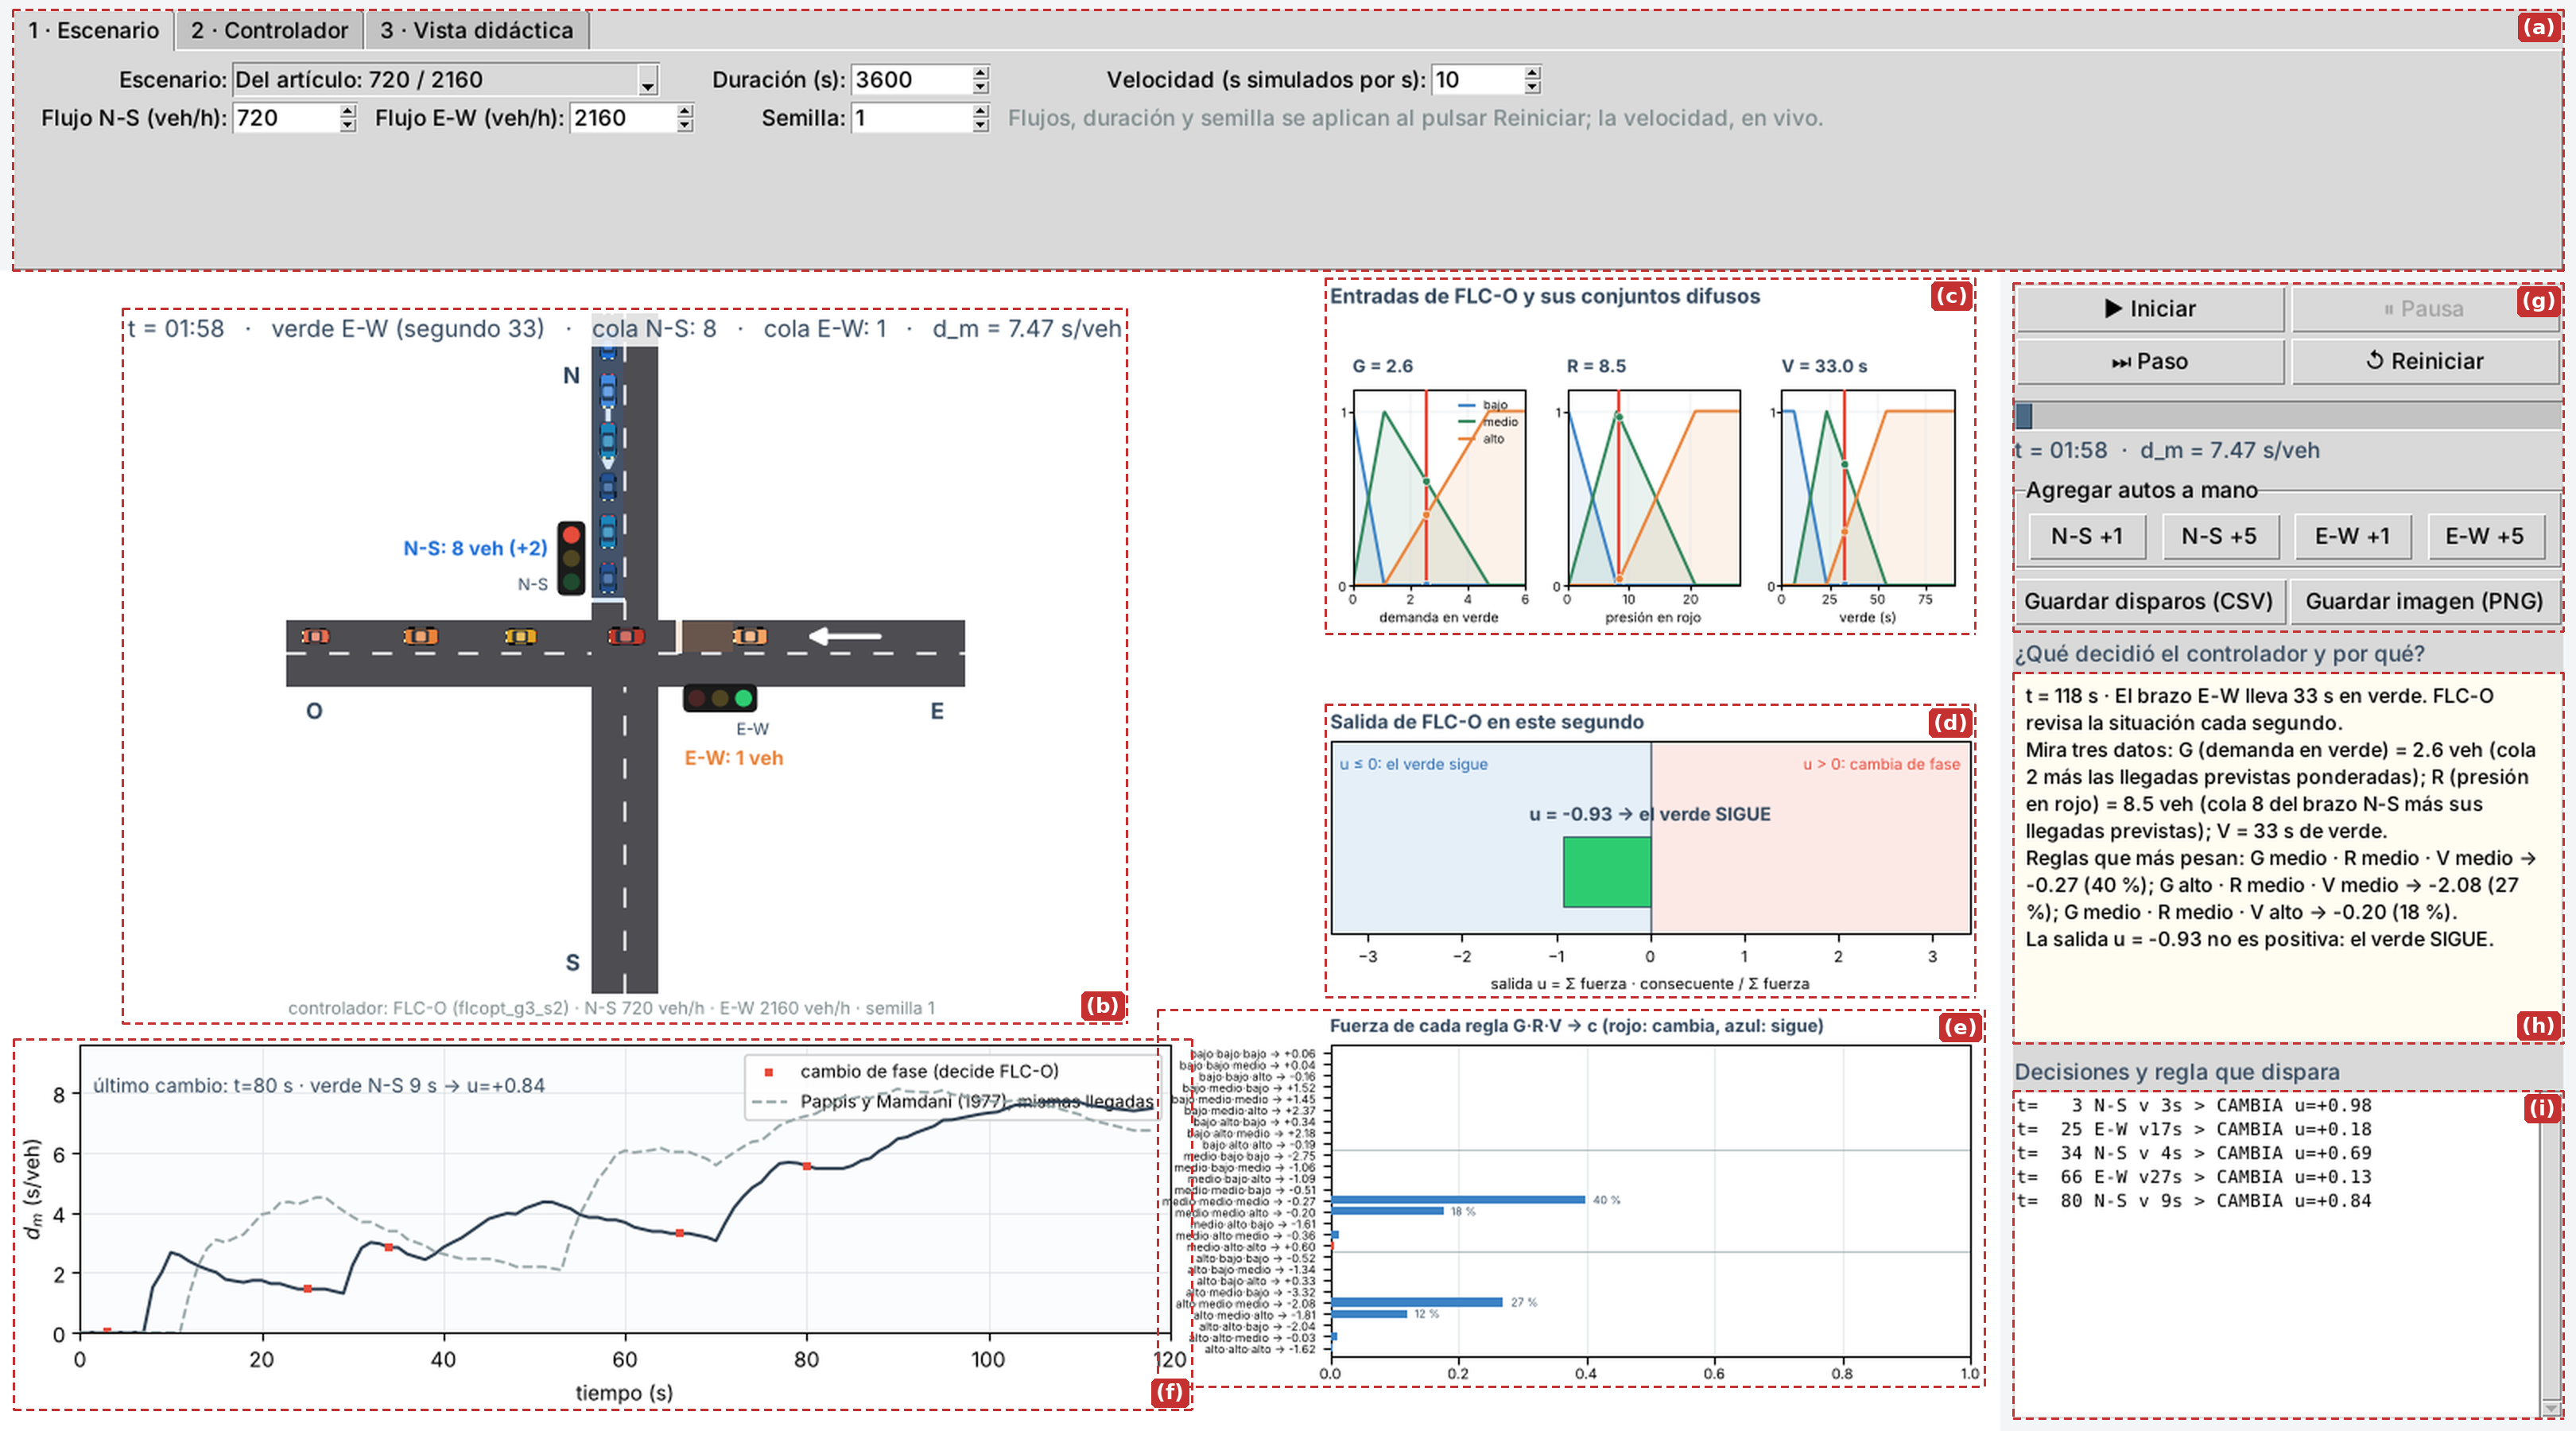
\includegraphics[width=\textwidth]{fig_sup_ventana_flco.png}
\caption{Simulador interactivo con \FLC{} (720/2160\,veh/h, semilla 1, $t=118$\,s). (a) Configuración: escenario, controlador y vista; (b) la intersección: vehículos (azules: N-S; cálidos: E-W), semáforos, colas, tiempo y retardo; (c) entradas $G$, $R$ y $V$ sobre sus conjuntos difusos; (d) salida $u$ de este segundo; (e) fuerza de cada una de las 27 reglas; (f) retardo medio en el tiempo, con la curva de \PMR{} sobre las mismas llegadas (punteada); (g) botones; (h) explicación de la decisión; (i) registro de cambios de fase. Captura de la ventana real; cada apartado se detalla en la Sec.~XII del suplemento.}
\label{fig:simulador}
\end{figure*}

\subsection{Cota óptima por programación dinámica}
\label{sec:pd}
Para saber cuánto puede mejorarse sin ver el futuro se calcula la política óptima de un proceso de decisión de Markov \cite{Puterman1994} con un paso de 1\,s. El estado es $(Q_1,Q_2,\text{fase})$ en verde, o $(Q_1,Q_2,\text{fase destino},k)$ con $k=1,\dots,4$ segundos ya perdidos; la acción en verde es continuar o cambiar; el costo por paso es $Q_1+Q_2$ y las llegadas son de Bernoulli con las tasas conocidas. La política minimiza el costo medio por segundo (iteración de valor relativa, colas truncadas a 80) y, por la ley de Little \cite{Little1961}, $L=\lambda W$, con $L$ la suma media de colas y $\lambda=\qbar_1+\qbar_2$ la tasa total de llegada, el retardo medio es $W=L/\lambda$, es decir, ese costo dividido por la tasa total. No hay mínimo ni máximo de verde. Es una cota para controladores que conocen los caudales y no ven llegadas futuras; no es realizable, pues los caudales no se conocen. Su validez se comprueba contra la simulación: en los 16 pares de la Tabla VIII, el retardo que predice la programación dinámica y el que se mide al simular su política difieren como máximo \PdMaxDif\,\%.

% =============================================================================
\section{Controladores optimizados}
\label{sec:opt}

Hay dos decisiones sobre las reglas. Primera: el controlador de 1977 se conserva \emph{sin cambios}, con sus 25 reglas, sus conjuntos y sus operadores, como línea base, porque es el sistema que se quiere mejorar y cualquier modificación confundiría la comparación. Segunda: el original obtuvo sus reglas por prueba y error y modificó las reglas, no los conjuntos difusos, porque incluir los parámetros de las funciones de pertenencia como variables de decisión habría aumentado radicalmente la dimensión del problema (p.~714). Un optimizador evolutivo puede hoy ajustar decenas de parámetros a la vez, así que se estudian dos caminos: afinar los números del controlador de 1977 conservando sus 25 reglas (Sec.~\ref{sec:afinado}) y diseñar reglas nuevas, con otras variables y consecuentes numéricos, cuyos conjuntos difusos también se aprenden (Sec.~\ref{sec:flc}). La Sec.~\ref{sec:res-abl} mide lo que aporta cada camino.

\subsection{Pappis y Mamdani afinado}
\label{sec:afinado}
Conserva la estructura de las 25 reglas y afina 30 números: el umbral $\tau$ de \eqref{eq:decision}, una escala y un desplazamiento para $A$ y para $Q$ ($A'=\kappa_AA+o_A$, $Q'=\kappa_QQ+o_Q$; las tablas se interpolan linealmente) y un desplazamiento de $-4$ a $4$\,s del conjunto de tiempo de cada una de las 25 reglas. Con los valores del original reproduce exactamente al controlador replicado. Muestra cuánto se gana solo con ajustar.

\subsection{FLC-O}
\label{sec:flc}
\FLC{} es un controlador difuso nuevo que decide cada segundo, una vez transcurrido el verde mínimo $g_{\min}$, si se sigue en verde o se cambia de fase. Tiene tres variables lingüísticas:
\begin{align}
G&=Q_g+\textstyle\sum_{k=1}^{3}\omega_k\,W_g(l_k), & l&=(2,5,10)\ \text{s},\nonumber\\
R&=Q_r+\textstyle\sum_{k=1}^{3}\rho_k\,W_r(l'_k), & l'&=(3,6,10)\ \text{s},\label{eq:GR}
\end{align}
y $V$, los segundos de verde transcurridos. Aquí $Q_g$ y $Q_r$ son las colas de los brazos con verde y en rojo, $W_g(l)$ y $W_r(l)$ las llegadas previstas en los $l$ segundos siguientes, y $\omega_k,\rho_k\ge0$ pesos que se aprenden: el entrenamiento elige cuánto mirar hacia adelante en lugar de fijarlo. $G$ es la demanda que aún puede aprovechar el verde y $R$, la presión que se acumula en el rojo. Cada variable tiene tres conjuntos (bajo, medio, alto) en una partición de Ruspini \cite{Ruspini1969} definida por tres nudos $k_1<k_2<k_3$ propios de la variable:
\begin{align}
\mu_{\text{bajo}}(x)&=\operatorname{sat}\Bigl(\tfrac{k_2-x}{k_2-k_1}\Bigr),\nonumber\\
\mu_{\text{alto}}(x)&=\operatorname{sat}\Bigl(\tfrac{x-k_2}{k_3-k_2}\Bigr),\label{eq:mf}\\
\mu_{\text{medio}}(x)&=1-\mu_{\text{bajo}}(x)-\mu_{\text{alto}}(x),\nonumber
\end{align}
con $\operatorname{sat}(z)=\min\{1,\max\{0,z\}\}$ (definiciones propias; las tres pertenencias suman 1 para todo $x$). «Bajo» vale 1 hasta $k_1$ y baja linealmente a 0 en $k_2$; «medio» es un triángulo de base $[k_1,k_3]$ con pico 1 en $k_2$; «alto» vale 1 desde $k_3$. Fuera de $[k_1,k_3]$ las pertenencias son $(1,0,0)$ por debajo y $(0,0,1)$ por encima: los conjuntos extremos son hombros, no queda ningún valor sin pertenencia, y como $G$, $R$ y $V$ no son negativas ni tienen tope, no hay comportamiento fuera del universo que definir. Para que siempre cumplan $k_1<k_2<k_3$, los nudos se parametrizan con tres números libres $(p_1,p_2,p_3)$ por variable: $k_1=|p_1|$, $k_2=k_1+|p_2|+0.05$ y $k_3=k_2+|p_3|+0.05$. Los valores del modelo elegido están en la Tabla~\ref{tab:reglasflc} y los 42 parámetros completos, en el suplemento. Las 27 reglas son
\begin{equation}
\text{si } G \text{ es } \mathcal{G}_i \text{ y } R \text{ es } \mathcal{R}_j \text{ y } V \text{ es } \mathcal{V}_k \text{ entonces } c_{ijk}\in\mathbb{R},
\label{eq:reglaflc}
\end{equation}
con consecuentes numéricos (conjuntos de salida de un solo punto). Con $w_{ijk}=\mu_{\mathcal{G}_i}(G)\,\mu_{\mathcal{R}_j}(R)\,\mu_{\mathcal{V}_k}(V)$ (producto como «y»), la salida $u$ es el promedio ponderado de los consecuentes y se cambia de fase si es positiva:
\begin{equation}
u=\frac{\sum_{ijk}w_{ijk}\,c_{ijk}}{\sum_{ijk}w_{ijk}},\qquad \text{cambiar}\iff u>0 .
\label{eq:salida}
\end{equation}
La salida \eqref{eq:salida} es el centro de gravedad de consecuentes de un solo punto, un sistema de Mamdani con salidas singleton equivalente a uno de Takagi y Sugeno de orden cero \cite{TakagiSugeno1985}. La combinación lineal de llegadas previstas en \eqref{eq:GR} es un diseño propio que generaliza el recuento de arribos $a_e$ del original: con un solo peso no nulo se recupera un horizonte fijo. A diferencia del de 1977 no tiene intervenciones cada 10\,s ni umbral de grado 0.5: decide cada segundo y el verde máximo es $g_{\max}$. Los parámetros son 9 nudos, 27 consecuentes y 6 pesos: 42 en total. En el modelo final $g_{\min}=3$\,s y $g_{\max}=90$\,s; el verde mínimo se eligió entre 3, 4, 5 y 7\,s con los escenarios de validación (Sección~\ref{sec:res-abl}). El resultado es legible (Fig.~\ref{fig:difuso} y Tabla~\ref{tab:reglasflc}): cada regla dice si, para esa demanda, esa presión y ese tiempo en verde, conviene cambiar o seguir.

\begin{figure*}[!t]
\centering
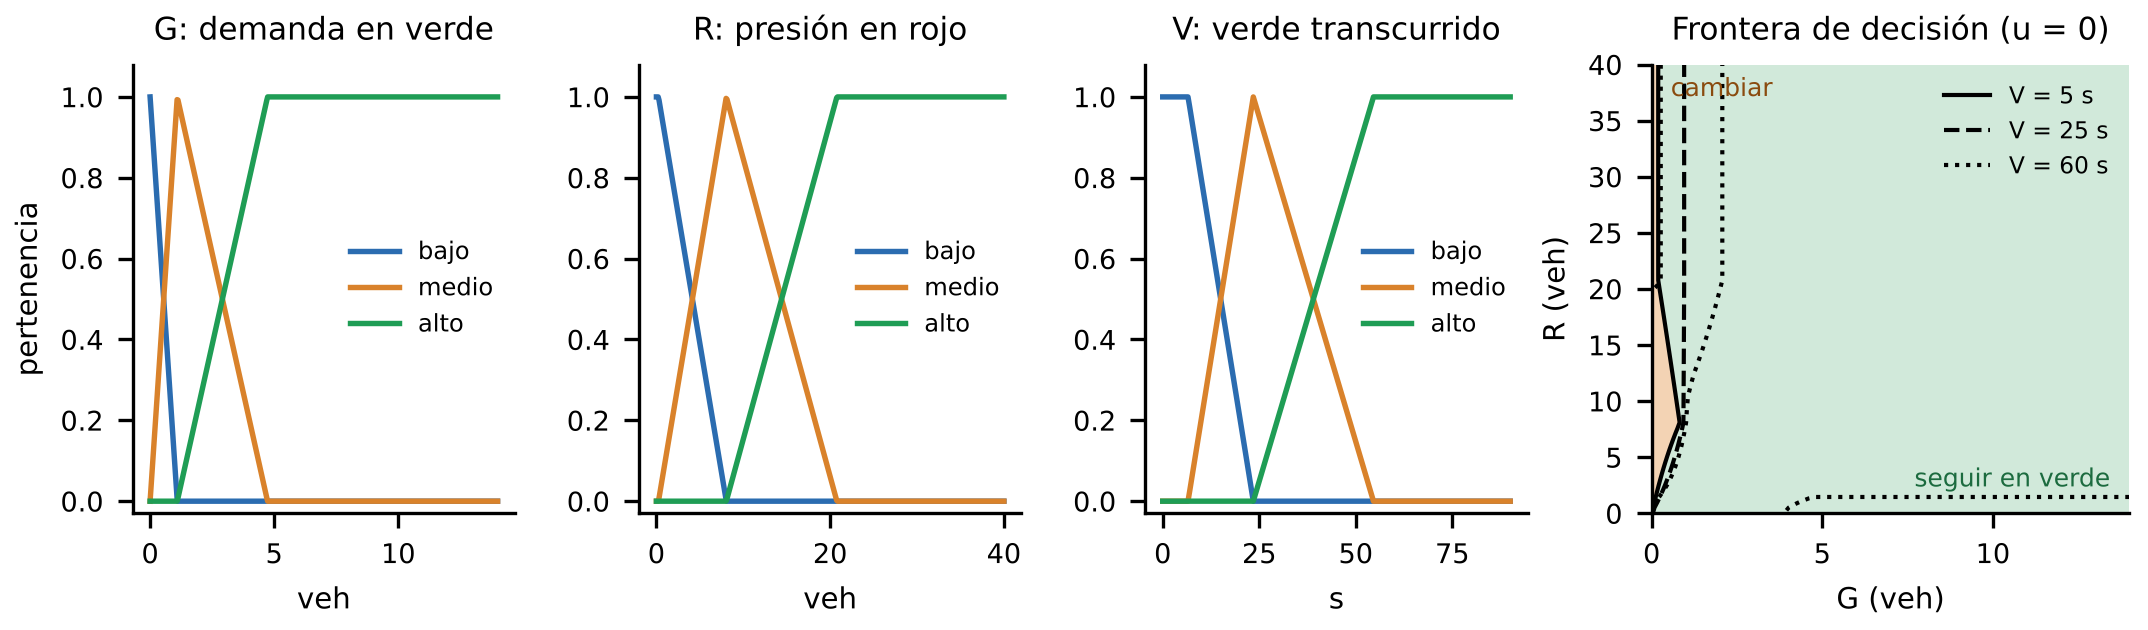
\includegraphics[width=\textwidth]{fig_opt_difuso.png}
\caption{Funciones de pertenencia aprendidas de \FLC{} para $G$, $R$ y $V$ (Ec.~\eqref{eq:mf} con los nudos de la Tabla~\ref{tab:reglasflc}; fuera de $[k_1,k_3]$ los conjuntos extremos valen 1) y frontera de decisión $u=0$ en el plano $(G,R)$ para tres valores de $V$.}
\label{fig:difuso}
\end{figure*}

\begin{table}[t]
\centering
\caption{Base de reglas de FLC-O: consecuente num\'erico $c_{ijk}$ de cada regla (positivo: cambiar la fase; negativo: seguir en verde) seg\'un la demanda en verde $G$, la presi\'on en rojo $R$ y el verde transcurrido $V$. Nudos $(k_1,k_2,k_3)$: $G$ (0.000, 1.095, 4.731), $R$ (0.239, 8.048, 20.776), $V$ (6.562, 23.457, 54.569). Pesos aprendidos de la vista adelante: verde (0.88, 0.21, 0.03) para 2, 5 y 10 s; rojo (0.22, 0.88, 0.49) para 3, 6 y 10 s.}
\label{tab:reglasflc}
\scriptsize
\begin{tabular}{@{}llrrr@{}}
\toprule
$G$ & $R$ & $V$ bajo & $V$ medio & $V$ alto \\
\midrule
bajo & bajo & +0.06 & +0.04 & $-$0.16 \\
bajo & medio & +1.52 & +1.45 & +2.37 \\
bajo & alto & +0.34 & +2.18 & $-$0.19 \\
medio & bajo & $-$2.75 & $-$1.06 & $-$1.09 \\
medio & medio & $-$0.51 & $-$0.27 & $-$0.20 \\
medio & alto & $-$1.61 & $-$0.36 & +0.60 \\
alto & bajo & $-$0.52 & $-$1.34 & +0.33 \\
alto & medio & $-$3.32 & $-$2.08 & $-$1.81 \\
alto & alto & $-$2.04 & $-$0.03 & $-$1.62 \\
\bottomrule
\end{tabular}
\fuente{modelo entrenado flcopt\_g3\_s2 (resultados/opt/flcopt\_g3\_s2.json).}
\end{table}


\subsection{Política neuronal}
\label{sec:neuronal}
Para saber qué tanto se pierde por exigir reglas legibles, se entrena también, con las mismas condiciones, una política opaca: un perceptrón de una capa oculta de 8 neuronas con tangente hiperbólica (121 parámetros) que recibe 12 características (colas, verde transcurrido, llegadas previstas en 3 y 10\,s, tasas de llegada de los últimos 5 y 20\,s, y si la cola del verde está vacía) y decide cada segundo. Es una referencia empírica de lo que logra un aprendizaje sin estructura con esa información; no es una cota, porque el entrenamiento puede quedar en un óptimo local, ni un controlador propuesto.

\subsection{Entrenamiento}
\label{sec:entrena}
Todos los parámetros se optimizan con CMA-ES \cite{Hansen2001,Hansen2016}: una estrategia evolutiva que adapta la covarianza de una distribución normal con la que sortea candidatos y que usa los mejores para actualizarla. El objetivo de un parámetro $\theta$ es
\begin{equation}
J(\theta)=\frac{1}{N}\sum_{i=1}^{N}\frac{d_m^{(i)}(\theta)}{d_m^{(i)}(\text{act})},
\label{eq:objetivo}
\end{equation}
la media sobre $N=64$ escenarios de entrenamiento (definición propia) del retardo \eqref{eq:dm} del controlador dividido por el del actuado afinado en el mismo escenario, de modo que $J<1$ significa mejor que el actuado y todos los niveles de demanda pesan igual. Los escenarios de entrenamiento son caudales sorteados al azar, con suma de 540 a 3300\,veh/h y semillas distintas de las de la prueba; no incluyen los 16 pares de la Tabla VIII. Cada evaluación simula 3600\,s por escenario. Con 4 procesos en paralelo (cuatro vCPU Intel Xeon a 2.10\,GHz, 15\,GB de memoria), entrenar \FLC{} toma unos 13 minutos (787\,s el modelo elegido).

% =============================================================================
\section{Protocolo experimental}
\label{sec:protocolo}

\textbf{Controladores comparados} (Tabla~\ref{tab:controladores}). «\PMR{}» es el controlador de 1977 con sus 25 reglas, conjuntos y operadores impresos y las entradas $A$ y $Q$ definidas en la Sección~\ref{sec:lecturas}; es una reconstrucción, no el programa original, y reproduce la Tabla~VIII impresa con un error medio de 9.2\,\%. Además de él, de su versión afinada y de \FLC{}: el ciclo fijo de Webster; el actuado por detector de la réplica (verde mínimo 7\,s, máximo 57\,s, hueco 3\,s); un actuado afinado, cuyo hueco, verde mínimo y máximo se eligieron en los mismos escenarios de entrenamiento y dentro del mismo rango que los controladores entrenados (verde mínimo de 3 a 7\,s, máximo de 90\,s): resultó hueco de 1\,s, mínimo de 3\,s y máximo de 90\,s, para que el rival sea justo; un actuado afinado \emph{con vista adelante}, que recibe la misma información que \PMR{} y \FLC{} (las llegadas de los próximos 10\,s): termina el verde cuando, pasado el mínimo, el brazo con verde no tiene cola ni se esperan llegadas en una ventana de $g$ s, y en el brazo en rojo hay cola o se esperan llegadas en una ventana de $g'$ s; sus cuatro parámetros ($g$ de 1 a 10\,s, $g'$ de 0, 3 o 6\,s, verde mínimo de 3 a 7\,s y máximo de 57, 80 o 90\,s) se eligieron igual, y resultaron $g=2$\,s, $g'=3$\,s, mínimo de 3\,s y máximo de 90\,s; la presión máxima \cite{Varaiya2013}, con parámetros afinados en el mismo rango; la cota óptima y la política neuronal. El actuado con vista adelante separa la ventaja de la información de la ventaja del método.

\begin{table}[t]
\centering
\caption{Controladores comparados y la información que usan}
\label{tab:controladores}
\scriptsize
\setlength{\tabcolsep}{2.5pt}
\begin{tabular}{@{}lccc@{}}
\toprule
Controlador & Caudales & Vista adelante & Parámetros \\
\midrule
Ciclo fijo (Webster) & sí & no & 0 \\
Actuado, actuado afinado & no & no & 3 \\
Actuado afinado con vista adelante & no & 10 s & 4 \\
Presión máxima & no & no & 3 \\
Pappis y Mamdani reconstruido & no & 10 s & 0 \\
Pappis y Mamdani reconstruido afinado & no & 10 s & 30 \\
Óptimo (programación dinámica) & sí & no & -- \\
FLC-O & no & 10 s (pesos aprendidos) & 42 \\
Política neuronal & no & 10 s & 121 \\
\bottomrule
\end{tabular}
\fuente{elaboración propia.}
\end{table}

\textbf{Conjuntos de prueba} (nunca usados para entrenar), todos de 7200\,s:
\begin{itemize}
\item \emph{Oficial}: los 16 pares de caudales de la Tabla VIII del original con 20 réplicas (semillas 0 a 19, números aleatorios comunes entre controladores).
\item \emph{No vistos}: 64 pares sorteados, un escenario por par (semillas 500000 a 500063).
\item \emph{Variable}: 64 escenarios con demanda que cambia cada 600\,s con un factor de 0.4 a 1.6 (semillas 300000 a 300063); se evalúa cómo se comportan controladores que no conocen los caudales.
\item \emph{Saturado}: 32 pares con suma de 3000 a 3300\,veh/h, cerca de la capacidad (semillas 400000 a 400031).
\end{itemize}

\textbf{Estadística.} En el conjunto oficial, para cada par de caudales se compara cada controlador con cada referencia con la prueba de rangos con signo de Wilcoxon sobre las 20 réplicas pareadas, con la corrección de Holm sobre los 16 pares, y se reportan la media, la desviación estándar muestral y el intervalo de confianza de 95\,\% (t de Student). La mejora de un par es la reducción relativa del retardo medio. En los otros conjuntos cada escenario es un par de caudales con una réplica y los controladores ven las mismas llegadas: se reportan la media con su intervalo de confianza de 95\,\% (t de Student sobre los escenarios), la reducción relativa media por escenario con su intervalo y el $p$ de Wilcoxon pareado. Las variantes de la ablación se entrenan con tres semillas de CMA-ES y se reportan la media y la desviación estándar muestral entre semillas. Todo el código y los resultados están en el repositorio (Sección~\ref{sec:disp}).

% =============================================================================
\section{Resultados}
\label{sec:resultados}

\subsection{Conjunto oficial: Tabla VIII}
\label{sec:res-oficial}
La Tabla~\ref{tab:oficial} y la Fig.~\ref{fig:retardo} muestran el retardo en los 16 pares. El retardo medio es de \DelayOfFijo{}\,s/veh con el ciclo fijo, \DelayOfPap{} con \PMR{}, \DelayOfActAf{} con el actuado afinado, \DelayOfActV{} con el actuado afinado con vista adelante y \DelayOfFlc{} con \FLC{}, es decir, una reducción de \RedFlc\,\% respecto de \PMR{}. Por par de caudales, la mejora media es de \ParMediaPap\,\% (de \ParMinPap\,\% a \ParMaxPap\,\%) y es significativa en \ParMejorPap{} de 16 pares, sin ningún par significativamente peor (Tabla~\ref{tab:comparaciones}). Frente al actuado afinado, la mejora media es de \ParMediaActAf\,\% (significativa en \ParMejorActAf{} pares y en contra en \ParPeorActAf{}), pero ese rival no ve las llegadas de los próximos segundos. Con la misma vista adelante, el actuado afinado baja de \DelayOfActAf{} a \DelayOfActV{} (\RedVistaAfOf\,\%) y la mejora de \FLC{} cae a \ParMediaActV\,\% por par (\RedActVOf\,\% sobre el promedio), significativa en \ParMejorActV{} de 16 pares y en contra en \ParPeorActV{}: la mayor parte de la ventaja sobre el actuado afinado era información, no método. El actuado con vista adelante, además, mejora en \RedVistaPapOf\,\% a \PMR{}: una parte grande de la distancia al controlador de 1977 se recorre con un controlador simple que recibe la misma información. La cota óptima, que conoce los caudales pero no ve el futuro, da \DelayOfMdp{}\,s/veh; \FLC{} queda por debajo de ella porque sí ve las llegadas de los próximos segundos, y no porque la cota sea defectuosa.

\begin{table*}[!t]
\centering
\caption{Retardo medio por veh\'iculo (s) $\pm$ desviaci\'on est\'andar muestral ($n-1$) de las 20 r\'eplicas, en los 16 pares de caudales de la Tabla VIII del art\'iculo original (7200 s, n\'umeros aleatorios comunes). Se cuenta la espera de todos los veh\'iculos hasta el horizonte. ``Pappis reconst.'': controlador de 1977 reconstruido (Sec.~\ref{sec:lecturas}). ``Actuado af. + vista'': actuado afinado con la misma vista adelante de 10 s que FLC-O. $\Delta_P$ y $\Delta_V$: mejora de FLC-O (\%) frente a Pappis reconst. y frente al actuado af. + vista; $^{*}$: significativa (Wilcoxon pareado, Holm, 0.05). En negrita, el menor retardo medio entre los controladores realizables.}
\label{tab:oficial}
\scriptsize
\setlength{\tabcolsep}{3pt}
\begin{tabular}{@{}lrrrrrrrr@{}}
\toprule
N-S / E-W (veh/h) & Webster & Actuado af. & Actuado af. + vista & Pappis reconst. & FLC-O & $\Delta_P$ (\%) & $\Delta_V$ (\%) & \'Optimo$^{\dagger}$ \\
\midrule
360 / 360 & 7.30 $\pm$ 0.17 & 5.30 $\pm$ 0.18 & 3.82 $\pm$ 0.16 & 5.58 $\pm$ 0.14 & \textbf{2.83 $\pm$ 0.10} & +49.3$^{*}$ & +26.0$^{*}$ & 5.01 \\
360 / 720 & 7.49 $\pm$ 0.15 & 5.90 $\pm$ 0.19 & 4.43 $\pm$ 0.17 & 5.97 $\pm$ 0.11 & \textbf{3.60 $\pm$ 0.13} & +39.8$^{*}$ & +18.8$^{*}$ & 5.61 \\
360 / 1080 & 7.77 $\pm$ 0.24 & 6.42 $\pm$ 0.18 & 4.89 $\pm$ 0.15 & 6.25 $\pm$ 0.11 & \textbf{4.12 $\pm$ 0.10} & +34.2$^{*}$ & +15.9$^{*}$ & 5.86 \\
360 / 1440 & 8.26 $\pm$ 0.32 & 7.03 $\pm$ 0.15 & 5.45 $\pm$ 0.15 & 6.70 $\pm$ 0.11 & \textbf{4.68 $\pm$ 0.14} & +30.1$^{*}$ & +14.0$^{*}$ & 6.26 \\
360 / 1800 & 9.22 $\pm$ 0.26 & 7.76 $\pm$ 0.18 & 6.10 $\pm$ 0.22 & 7.40 $\pm$ 0.22 & \textbf{5.49 $\pm$ 0.20} & +25.8$^{*}$ & +9.9$^{*}$ & 6.90 \\
360 / 2160 & 11.34 $\pm$ 1.32 & 8.68 $\pm$ 0.18 & 7.09 $\pm$ 0.24 & 8.71 $\pm$ 0.29 & \textbf{6.62 $\pm$ 0.28} & +24.0$^{*}$ & +6.7$^{*}$ & 7.99 \\
360 / 2520 & 16.31 $\pm$ 4.56 & 10.42 $\pm$ 0.35 & 9.17 $\pm$ 0.50 & 12.02 $\pm$ 0.73 & \textbf{9.06 $\pm$ 0.50} & +24.7$^{*}$ & +1.3$^{*}$ & 9.95 \\
720 / 720 & 9.36 $\pm$ 0.14 & 7.13 $\pm$ 0.14 & 5.52 $\pm$ 0.13 & 6.57 $\pm$ 0.15 & \textbf{4.87 $\pm$ 0.11} & +25.9$^{*}$ & +11.8$^{*}$ & 7.04 \\
720 / 1080 & 10.65 $\pm$ 0.21 & 8.05 $\pm$ 0.15 & 6.47 $\pm$ 0.14 & 7.54 $\pm$ 0.16 & \textbf{6.00 $\pm$ 0.11} & +20.5$^{*}$ & +7.3$^{*}$ & 7.88 \\
720 / 1440 & 12.53 $\pm$ 0.42 & 9.15 $\pm$ 0.18 & 7.65 $\pm$ 0.20 & 9.34 $\pm$ 0.29 & \textbf{7.37 $\pm$ 0.18} & +21.1$^{*}$ & +3.7$^{*}$ & 9.01 \\
720 / 1800 & 15.38 $\pm$ 0.46 & 10.82 $\pm$ 0.30 & 9.48 $\pm$ 0.35 & 12.21 $\pm$ 0.50 & \textbf{9.35 $\pm$ 0.37} & +23.5$^{*}$ & +1.4$^{*}$ & 10.70 \\
720 / 2160 & 21.27 $\pm$ 0.78 & 13.66 $\pm$ 0.59 & 12.97 $\pm$ 0.63 & 17.69 $\pm$ 1.36 & \textbf{12.89 $\pm$ 0.70} & +27.1$^{*}$ & +0.6 & 13.63 \\
1080 / 1080 & 13.56 $\pm$ 0.28 & 9.58 $\pm$ 0.20 & 8.14 $\pm$ 0.17 & 9.78 $\pm$ 0.31 & \textbf{7.87 $\pm$ 0.19} & +19.5$^{*}$ & +3.3$^{*}$ & 9.58 \\
1080 / 1440 & 17.81 $\pm$ 0.42 & 11.81 $\pm$ 0.30 & 10.68 $\pm$ 0.36 & 13.82 $\pm$ 0.53 & \textbf{10.53 $\pm$ 0.29} & +23.8$^{*}$ & +1.4$^{*}$ & 11.79 \\
1080 / 1800 & 25.68 $\pm$ 0.87 & 15.85 $\pm$ 0.58 & 15.41 $\pm$ 0.68 & 22.41 $\pm$ 1.95 & \textbf{15.33 $\pm$ 0.72} & +31.6$^{*}$ & +0.5 & 15.89 \\
1440 / 1440 & 26.98 $\pm$ 1.00 & 16.48 $\pm$ 0.69 & 16.13 $\pm$ 0.77 & 23.24 $\pm$ 1.91 & \textbf{16.00 $\pm$ 0.78} & +31.2$^{*}$ & +0.9$^{*}$ & 16.44 \\
\midrule
Media de los 16 pares & 13.81 & 9.63 & 8.34 & 10.95 & 7.91 & +28.2 & +7.7 & 9.35 \\
\bottomrule
\end{tabular}
\fuente{simulaci\'on del autor (resultados/opt/evaluacion\_final.json); $^{\dagger}$ cota por programaci\'on din\'amica que conoce los caudales y no ve llegadas futuras (Sec.~\ref{sec:pd}); es determinista, sin dispersi\'on.}
\end{table*}

\begin{table}[t]
\centering
\caption{FLC-O frente a cada referencia en la Tabla VIII. Mejora media del retardo por par de caudales (\%); IC de 95\,\% de esa media (t de Student sobre las 16 mejoras por par); rango (m\'inimo a m\'aximo) de las 16 mejoras, que no es un intervalo de confianza; y n\'umero de pares (de 16) en que FLC-O es significativamente mejor o peor (Wilcoxon pareado sobre 20 r\'eplicas, correcci\'on de Holm, 0.05).}
\label{tab:comparaciones}
\scriptsize
\setlength{\tabcolsep}{2.6pt}
\begin{tabular}{@{}lrrrrr@{}}
\toprule
Referencia & Media & IC 95\,\% & Rango & Mejor & Peor \\
\midrule
Pappis y Mamdani reconstruido & +28.2 & [+24.1, +32.4] & +19.5 a +49.3 & 16 & 0 \\
Ciclo fijo (Webster) & +44.1 & [+41.0, +47.1] & +39.2 a +61.2 & 16 & 0 \\
Actuado (hueco 3 s) & +31.3 & [+23.5, +39.1] & +11.4 a +56.8 & 16 & 0 \\
Actuado afinado & +22.0 & [+14.9, +29.1] & +2.9 a +46.5 & 16 & 0 \\
Actuado afinado con vista adelante & +7.7 & [+3.6, +11.8] & +0.5 a +26.0 & 14 & 0 \\
Óptimo (PD, caudales conocidos) & +19.2 & [+12.9, +25.5] & +2.7 a +43.5 & 16 & 0 \\
\bottomrule
\end{tabular}
\fuente{simulaci\'on del autor; Wilcoxon exacto o con aproximaci\'on normal seg\'un empates (estadistica.py).}
\end{table}


\begin{figure*}[!t]
\centering
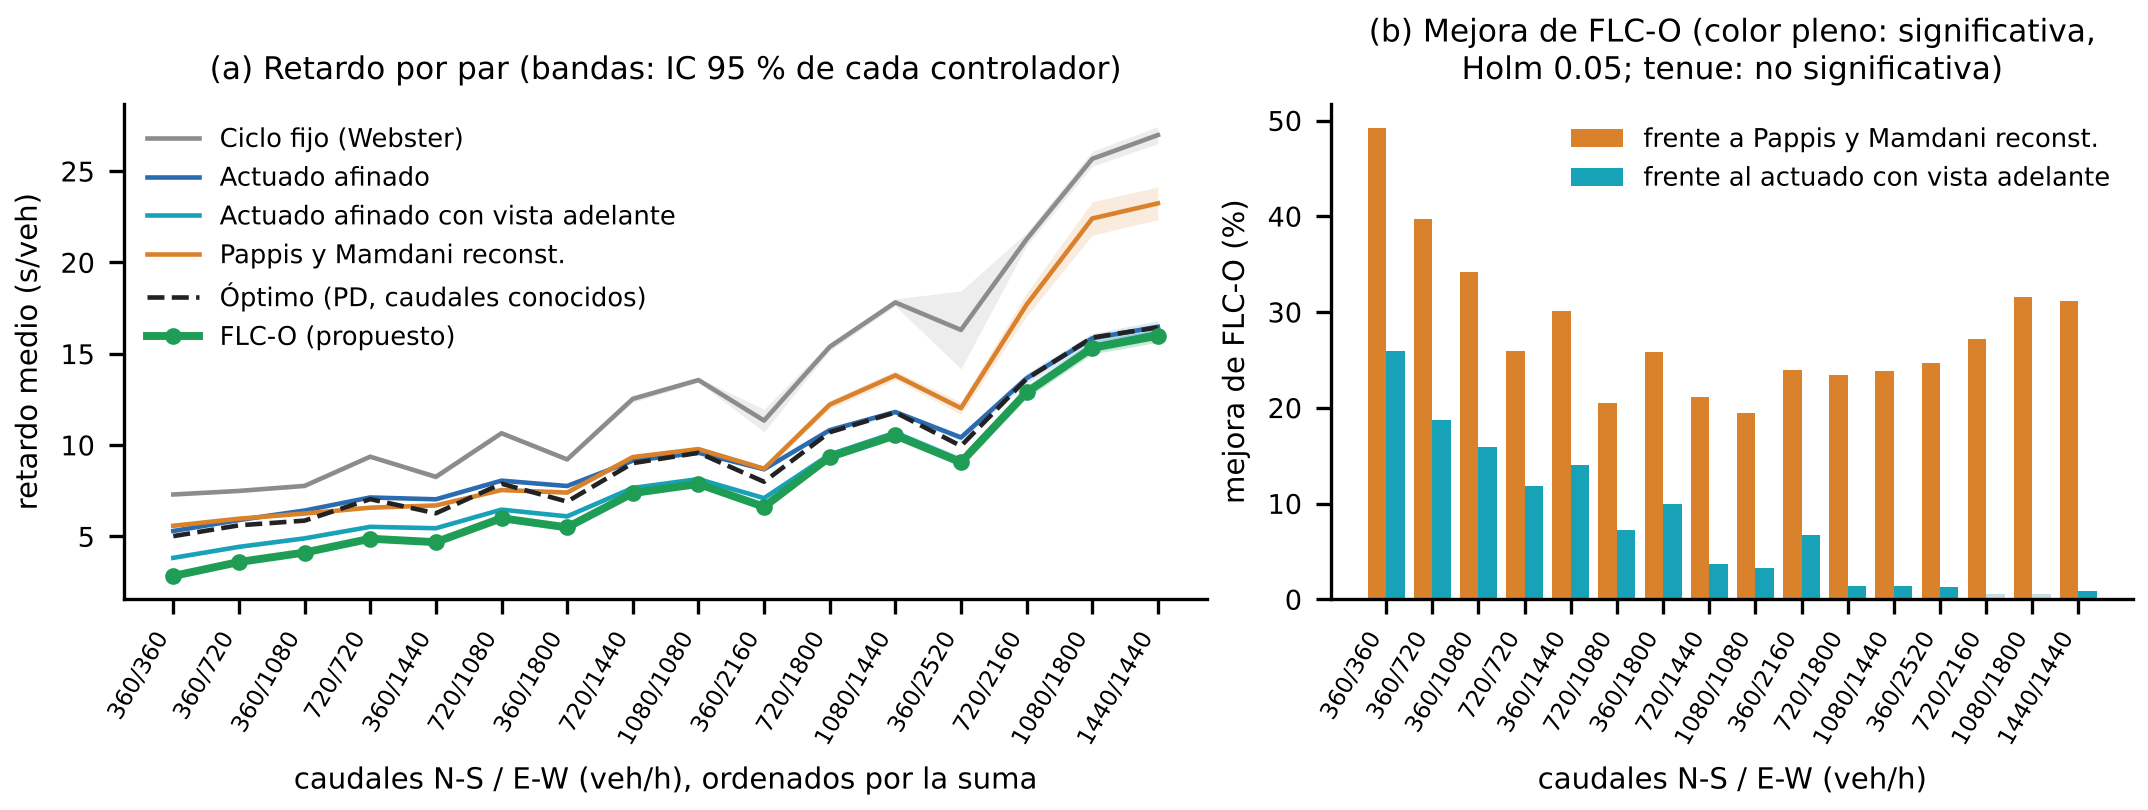
\includegraphics[width=\textwidth]{fig_opt_retardo.png}
\caption{(a) Retardo medio por par de caudales de la Tabla VIII (7200\,s, 20 réplicas); cada banda es el intervalo de confianza de 95\,\% de las 20 réplicas del controlador de su color (la cota óptima es determinista y no tiene banda). (b) Mejora de \FLC{} frente a \PMR{} y frente al actuado afinado con vista adelante en cada par; color pleno: significativa con la corrección de Holm; tenue: no significativa.}
\label{fig:retardo}
\end{figure*}

\subsection{Caudales no vistos, demanda variable y saturación}
\label{sec:res-otros}
La Tabla~\ref{tab:conjuntos} resume los otros conjuntos, con el número de unidades, el intervalo de confianza de cada media y la reducción de \FLC{} por unidad. Con 64 pares de caudales no vistos, \FLC{} reduce el retardo en \RedPapNv\,\% frente a \PMR{}, en \RedActAfNv\,\% frente al actuado afinado y en \RedActVNv\,\% frente al actuado con vista adelante (por escenario, \EscActVNvRed\,\%, IC 95\,\% de \EscActVNvLo\,\% a \EscActVNvHi\,\%, $p$ \EscActVNvP{}, mejor en \EscActVNvMejor{} de 64 y peor en \EscActVNvPeor{}), de modo que la mejora no depende de los 16 pares de la Tabla VIII. Con demanda variable, que es donde un controlador que adapta su decisión a lo que ve debería ganar más, las reducciones son de \RedPapVa\,\%, \RedActAfVa\,\% y \RedActVVa\,\%, y superan a las del caso estacionario. Cerca de la saturación, \FLC{} queda a la par del actuado afinado (\DelaySaFlc{} frente a \DelaySaActAf{}\,s/veh): la reducción por escenario es de \EscActAfSaRed\,\% (IC 95\,\% de \EscActAfSaLo\,\% a \EscActAfSaHi\,\%), mejor en \EscActAfSaMejor{} de 32 escenarios y peor en \EscActAfSaPeor{}, y el $p$ de Wilcoxon es \EscActAfSaP{}: no hay diferencia significativa, aunque con 32 escenarios no se puede afirmar que sean equivalentes. El actuado con vista adelante da \DelaySaActV{} y \FLC{} lo mejora en \EscActVSaRed\,\% ($p$ \EscActVSaP{}). \PMR{} da \DelaySaPap{}, con un verde máximo de 57\,s que limita su estructura; el ciclo fijo da \DelaySaFijo{}. Aquí \FLC{} no mejora al actuado afinado. El entrenamiento con caudales de hasta 3300\,veh/h fue lo que evitó la degradación observada en pruebas previas con caudales de hasta 3000.

\begin{table*}[!t]
\centering
\caption{Retardo medio (s/veh) $\pm$ semiancho del IC de 95\,\% en los cuatro conjuntos de prueba (todos de 7200 s), y reducci\'on de FLC-O por unidad frente a tres referencias. Unidad de an\'alisis y semillas de las llegadas: Oficial, los 16 pares de la Tabla VIII, cada uno con la media de 20 r\'eplicas (semillas 0 a 19); No vistos, 64 escenarios con caudales sorteados (semillas 500000 a 500063); Variable, 64 escenarios con demanda por tramos de 600 s y factor de 0.4 a 1.6 (semillas 300000 a 300063); Saturado, 32 escenarios con suma de caudales de 3000 a 3300 veh/h (semillas 400000 a 400031). Cada escenario es un par de caudales con una r\'eplica; los controladores ven las mismas llegadas.}
\label{tab:conjuntos}
\scriptsize
\setlength{\tabcolsep}{3pt}
\begin{tabular}{@{}lllll@{}}
\toprule
Controlador & Oficial ($n=16$ pares) & No vistos ($n=64$) & Variable ($n=64$) & Saturado ($n=32$) \\
\midrule
Ciclo fijo (Webster) & 13.8 $\pm$ 3.4 & 13.0 $\pm$ 1.4 & 12.3 $\pm$ 1.6 & 40.7 $\pm$ 3.1 \\
Actuado (hueco 3 s) & 10.9 $\pm$ 1.8 & 10.6 $\pm$ 0.8 & 9.2 $\pm$ 0.6 & 54.1 $\pm$ 16.3 \\
Actuado afinado & 9.6 $\pm$ 1.8 & 9.2 $\pm$ 0.8 & 8.1 $\pm$ 0.6 & 24.1 $\pm$ 2.1 \\
Actuado afinado con vista adelante & 8.3 $\pm$ 2.0 & 7.8 $\pm$ 0.8 & 6.6 $\pm$ 0.6 & 25.6 $\pm$ 2.7 \\
Presión máxima & 17.4 $\pm$ 1.7 & 16.5 $\pm$ 0.7 & 19.0 $\pm$ 0.6 & 152.3 $\pm$ 32.6 \\
Pappis y Mamdani reconstruido & 11.0 $\pm$ 3.0 & 10.4 $\pm$ 1.2 & 8.7 $\pm$ 1.0 & 105.9 $\pm$ 24.2 \\
Pappis y Mamdani reconstruido afinado & 9.7 $\pm$ 1.8 & 9.3 $\pm$ 0.7 & 8.1 $\pm$ 0.6 & 58.1 $\pm$ 17.9 \\
FLC-O (propuesto) & 7.9 $\pm$ 2.2 & 7.4 $\pm$ 0.9 & 6.1 $\pm$ 0.7 & 24.3 $\pm$ 2.3 \\
Óptimo (PD, caudales conocidos) & 9.3 $\pm$ 1.9 & 8.8 $\pm$ 0.8 & 7.9 $\pm$ 0.6 & -- \\
Política neuronal (referencia) & 8.1 $\pm$ 2.1 & 7.5 $\pm$ 0.9 & 6.2 $\pm$ 0.7 & 25.1 $\pm$ 2.9 \\
\midrule
\multicolumn{5}{l}{Reducci\'on media de FLC-O por unidad (\%) [IC 95\,\%], $p$ de Wilcoxon pareado} \\
\quad frente a Pappis y Mamdani reconstruido & 28.2 [24.1, 32.4], $p$ $<\!0.001$ & 29.7 [27.6, 31.8], $p$ $<\!0.001$ & 30.0 [28.3, 31.6], $p$ $<\!0.001$ & 69.5 [64.3, 74.7], $p$ $<\!0.001$ \\
\quad frente a Actuado afinado & 22.0 [14.9, 29.1], $p$ $<\!0.001$ & 23.3 [20.1, 26.5], $p$ $<\!0.001$ & 27.1 [24.8, 29.3], $p$ $<\!0.001$ & $-$0.3 [$-$1.3, 0.6], $p$ = 0.36 \\
\quad frente a Actuado afinado con vista adelante & 7.7 [3.6, 11.8], $p$ $<\!0.001$ & 7.9 [6.0, 9.8], $p$ $<\!0.001$ & 10.1 [8.8, 11.5], $p$ $<\!0.001$ & 4.4 [3.0, 5.9], $p$ $<\!0.001$ \\
\bottomrule
\end{tabular}
\fuente{simulaci\'on del autor (resultados/opt/evaluacion\_final.json). El \'optimo no se calcula en el conjunto saturado (la cola truncada de la programaci\'on din\'amica no es fiable all\'i) y es determinista (sin IC).}
\end{table*}


\subsection{Qué produce la mejora}
\label{sec:res-abl}
La Tabla~\ref{tab:ablacion} compara variantes entrenadas con las mismas condiciones, de modo que cada fila cambia un solo factor. Las filas con $n=3$ se entrenaron con tres semillas de CMA-ES y se reportan con su media y su desviación estándar entre semillas; las de $n=1$ son exploratorias, porque un solo entrenamiento no permite separar un efecto de la variación entre semillas.
(i) Afinar solo las 25 reglas de Pappis y Mamdani ($n=1$) da \DelayOfPapAf{}\,s/veh en el conjunto oficial: parte de la mejora viene del ajuste, pero no toda.
(ii) El verde mínimo es el factor que más pesa. Con $g_{\min}$ de 7, 5, 4 y 3\,s, \FLC{} da \MedOfGSiete{}, \MedOfGCinco{}, \MedOfGCuatro{} y \MedOfGTres{}\,s/veh (desviaciones estándar de \SdOfGSiete{}, \SdOfGCinco{}, \SdOfGCuatro{} y \SdOfGTres{}). Los pasos de 7 a 5\,s y de 5 a 4\,s superan varias veces la dispersión entre semillas (cada semilla de un valor queda por debajo de cada semilla del anterior). El paso de 4 a 3\,s, en cambio, es de solo $\approx$0.07\,s/veh, del orden de esa dispersión, y sus semillas se solapan: con 3\,s no se puede afirmar una ganancia frente a 4\,s. Con 5\,s se conserva casi toda la mejora (\RedPapMedGCinco\,\% frente a \PMR{} en promedio de las semillas, contra \RedPapMedGTres\,\% con 3\,s), lo que importa si la norma local exige un verde mínimo mayor.
(iii) Aprender los pesos de la vista adelante ayuda: con horizontes fijos, el mismo difuso de 27 reglas y 36 parámetros da \MedOfFijos{}\,s/veh (desviación estándar de \SdOfFijos{}) frente a \MedOfGTres{} de \FLC{}, y cada una de las tres semillas de \FLC{} queda por debajo de cada una de las tres de horizontes fijos.
(iv) Con una cuarta variable (el tiempo desde la última llegada) la base crece a 81 reglas, tres veces más, y da \MedOfReglas{}\,s/veh (desviación estándar de \SdOfReglas{}): no se distingue de las 27 reglas con horizontes fijos (\MedOfFijos{}). No se probaron bases de menos de 27 reglas.
(v) La política neuronal de 121 parámetros ($n=1$), entrenada igual, da \DelayOfMlp{}\,s/veh, no mejor que \FLC{}: exigir reglas legibles no cuesta desempeño aquí, aunque un solo entrenamiento no permite afirmar que la red no pueda superarlo, y la red no es una cota.
(vi) Sin vista adelante ($n=1$ en las tres), \FLC{} causal da \DelayOfFlcC{}\,s/veh, la política lineal con hueco \DelayOfLinC{} y la neuronal \DelayOfMlpC{}, frente a \DelayOfActAf{} del actuado afinado: la mejor, la neuronal, lo mejora solo en \RedActMlpC\,\% y \FLC{} causal queda en \RedActFlcC\,\%, contra \RedActAfOf\,\% de \FLC{} con vista adelante. La mayor parte de la mejora depende de ver el futuro cercano. Es coherente con lo que el original dice de su propio resultado: lo atribuye a colocar los detectores lejos de la línea de parada, a detectar ambos brazos a la vez y al conjunto de reglas obtenido por prueba y error (p.~715).

\begin{table*}[!t]
\centering
\caption{Variantes de FLC-O y controladores aprendidos, entrenados con las mismas condiciones. Retardo medio (s/veh) en la Tabla VIII, en caudales no vistos y con demanda variable. Con 3 semillas de entrenamiento (columna $n$), media $\pm$ desviaci\'on est\'andar muestral ($n-1$) entre semillas; con $n=1$, un solo entrenamiento (exploratorio, sin incertidumbre). $g_{\min}$: verde m\'inimo.}
\label{tab:ablacion}
\scriptsize
\setlength{\tabcolsep}{2.4pt}
\begin{tabular}{@{}lrlrrrr@{}}
\toprule
Variante & Par. & Informaci\'on & $n$ & Oficial & No vistos & Variable \\
\midrule
Pappis y Mamdani afinado (cada 10 s, $g_{\min}=7$) & 30 & vista adelante & 1 & 9.67 & 9.30 & 8.06 \\
Difuso 27 reglas, horizontes fijos ($g_{\min}=3$) & 36 & vista adelante & 3 & 8.47 $\pm$ 0.04 & 7.89 $\pm$ 0.03 & 6.56 $\pm$ 0.02 \\
Difuso 81 reglas con hueco ($g_{\min}=3$) & 93 & vista adelante & 3 & 8.44 $\pm$ 0.03 & 7.87 $\pm$ 0.05 & 6.55 $\pm$ 0.00 \\
FLC-O, $g_{\min}=7$ & 42 & vista adelante & 3 & 8.55 $\pm$ 0.05 & 8.11 $\pm$ 0.04 & 6.84 $\pm$ 0.02 \\
FLC-O, $g_{\min}=5$ & 42 & vista adelante & 3 & 8.19 $\pm$ 0.05 & 7.72 $\pm$ 0.08 & 6.44 $\pm$ 0.09 \\
FLC-O, $g_{\min}=4$ & 42 & vista adelante & 3 & 8.05 $\pm$ 0.02 & 7.56 $\pm$ 0.01 & 6.20 $\pm$ 0.04 \\
FLC-O, $g_{\min}=3$ & 42 & vista adelante & 3 & 7.98 $\pm$ 0.06 & 7.47 $\pm$ 0.06 & 6.18 $\pm$ 0.09 \\
Política neuronal ($g_{\min}=3$) & 121 & vista adelante & 1 & 8.09 & 7.53 & 6.24 \\
Difuso 27 reglas, causal & 36 & solo pasado & 1 & 9.97 & 9.37 & 8.41 \\
Política lineal causal con hueco & 16 & solo pasado & 1 & 9.53 & 8.97 & 8.10 \\
Política neuronal, causal & 121 & solo pasado & 1 & 9.46 & 8.95 & 8.05 \\
\textbf{FLC-O propuesto} (semilla elegida) & 42 & vista adelante & 1 & 7.91 & 7.40 & 6.07 \\
\bottomrule
\end{tabular}
\fuente{simulaci\'on del autor; par.: n\'umero de par\'ametros entrenados; las semillas cambian solo la semilla de CMA-ES, con los mismos escenarios de entrenamiento.}
\end{table*}


\begin{figure*}[!t]
\centering
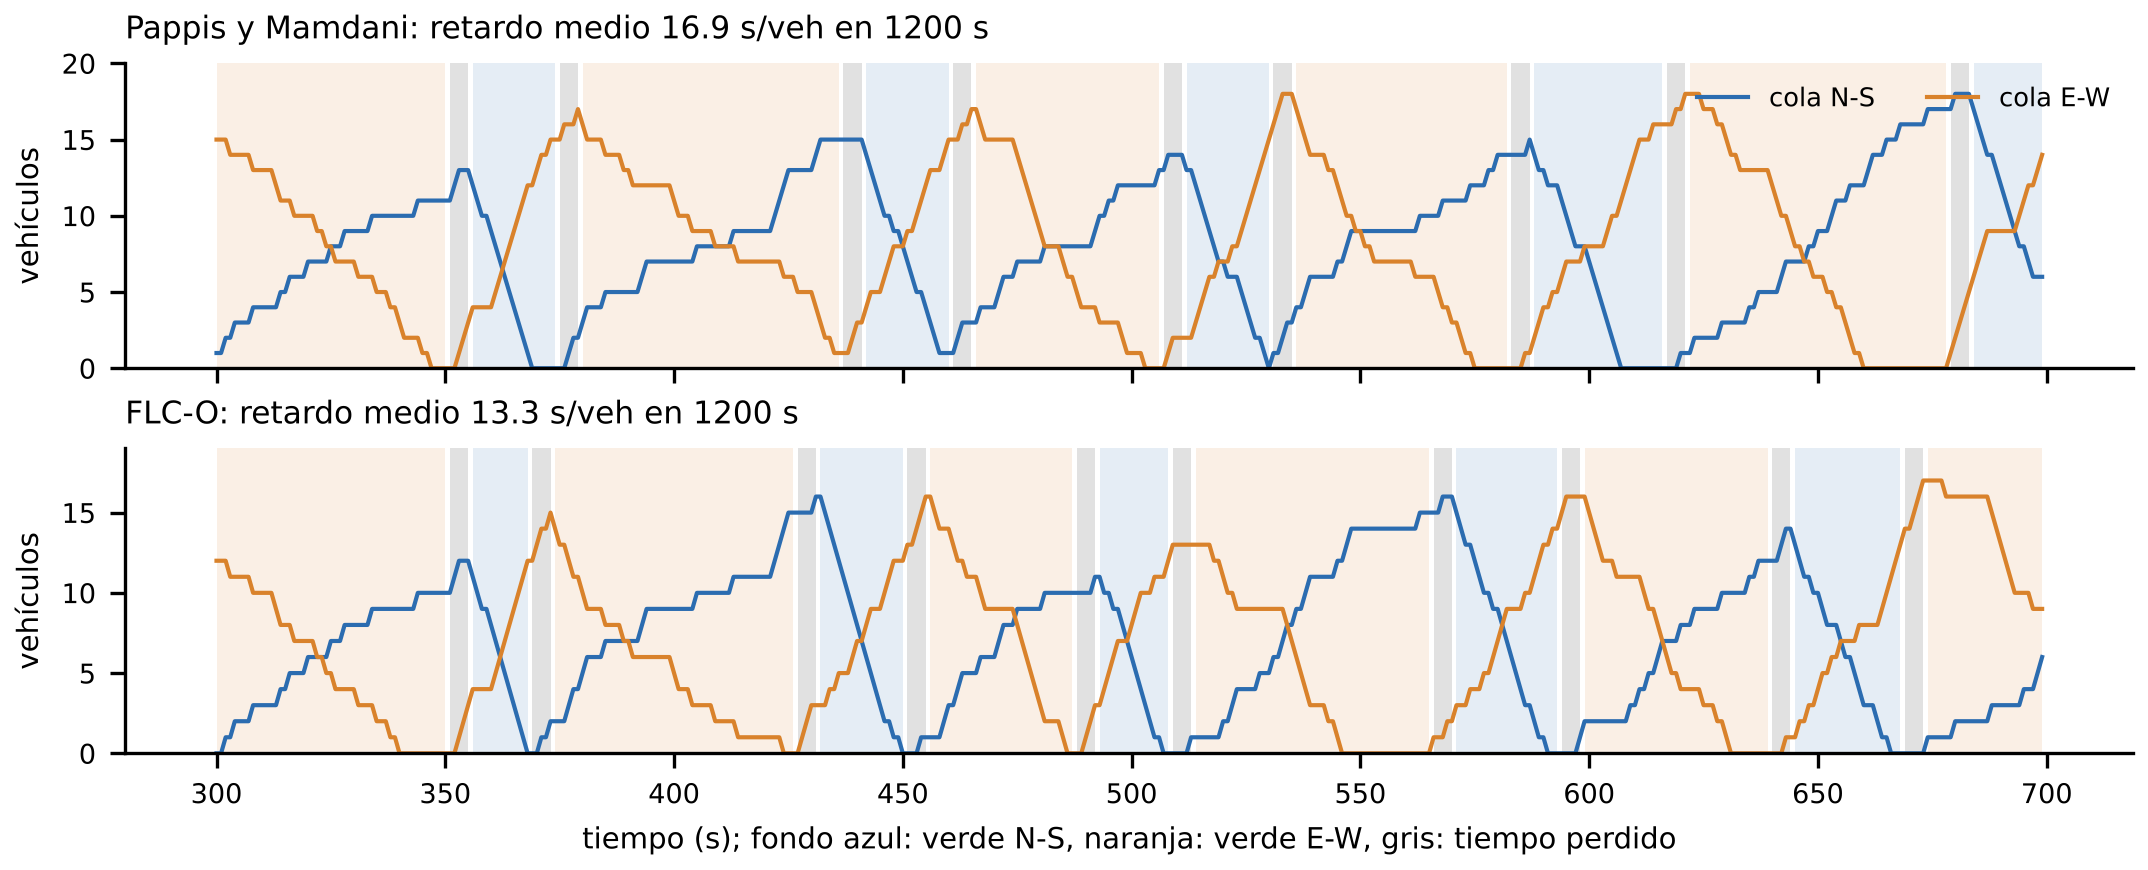
\includegraphics[width=\textwidth]{fig_opt_traza.png}
\caption{Colas y fases durante 400\,s en un escenario de 720/2160\,veh/h con las mismas llegadas: Pappis y Mamdani (arriba) y \FLC{} (abajo). El fondo indica el brazo con verde y, en gris, el tiempo perdido.}
\label{fig:traza}
\end{figure*}

% =============================================================================
\section{Discusión}
\label{sec:discusion}

\textbf{Qué se logró.} Dentro del modelo del original, un controlador difuso de 27 reglas y 42 parámetros entrenado con caudales sorteados reduce el retardo en \RedFlc\,\% frente a \PMR{} en la Tabla VIII, que tiene la misma vista adelante, y mejora en \RedActAfOf\,\% a un actuado afinado sin vista adelante y en \RedActVOf\,\% a uno con la misma vista adelante, que es la comparación que separa el método de la información. Las mejoras se mantienen con caudales no vistos (\RedPapNv\,\%, \RedActAfNv\,\% y \RedActVNv\,\%) y con demanda variable (\RedPapVa\,\%, \RedActAfVa\,\% y \RedActVVa\,\%). Según la ablación, las razones son tres: decide cada segundo y no cada 10\,s, admite un verde mínimo menor, y mide la demanda y la presión con pesos de la vista adelante aprendidos y no con las tablas fijas de 1977. Un resultado que conviene destacar: un actuado simple con la misma vista adelante ya mejora en \RedVistaPapOf\,\% al controlador de 1977; el aporte propio de \FLC{} es la ganancia que queda sobre ese actuado (\RedActVOf\,\%). La variación entre semillas de entrenamiento es pequeña (media \MedOfGTres{}\,s/veh con desviación estándar de \SdOfGTres{}, Tabla~S6 del suplemento). El modelo elegido por validación es el mejor de las tres semillas; la reducción media de las tres frente a \PMR{} es de \RedPapMedGTres\,\%, un poco menor que la del modelo elegido (\RedFlc\,\%).

\textbf{Qué no se logró.} (i) La mayor parte de la mejora sobre el actuado afinado depende de la vista adelante de 10\,s. Es un supuesto del original, que equivale a detectores aguas arriba sin error de medición, y es optimista en la práctica. Con la misma vista adelante, la mejora sobre el actuado cae de \RedActAfOf\,\% a \RedActVOf\,\%. Sin ella, el mejor controlador aprendido mejora al actuado afinado solo en \RedActMlpC\,\% y el difuso causal no lo mejora. (ii) Cerca de la saturación \FLC{} no mejora al actuado afinado (\DelaySaFlc{} frente a \DelaySaActAf{}\,s/veh; $p$ de Wilcoxon \EscActAfSaP{}); su ventaja es sobre \PMR{} (\DelaySaPap{}), limitado por su verde máximo de 57\,s, y sobre el ciclo fijo (\DelaySaFijo{}). (iii) El verde mínimo de 3\,s elegido por validación puede no ser admisible en una intersección real, por seguridad y por la norma local; con 5\,s la ganancia es de \RedPapMedGCinco\,\% frente a \PMR{} (media de tres semillas). (iv) Todo es simulación con llegadas de Bernoulli, un solo cruce y un flujo de saturación fijo; no hay datos de campo, ni giros, ni peatones, ni redes. (v) Las cifras de \PMR{} salen de nuestra simulación del controlador, con las definiciones de $A$ y $Q$ de la Sección~\ref{sec:lecturas}, y no de la Tabla~VIII impresa, que se reproduce con un error medio de 9.2\,\% y máximo de 18.6\,\%: el original no da el número de réplicas ni el generador aleatorio. (vi) Las filas de la Tabla~\ref{tab:ablacion} con $n=1$ son exploratorias: un solo entrenamiento no permite separar un efecto de la variación entre semillas.

\textbf{Amenazas a la validez.} Los parámetros se entrenaron con el mismo simulador con el que se evalúan, aunque con caudales y semillas distintos; un simulador distinto, o datos reales, podrían cambiar las conclusiones. El actuado afinado, el actuado afinado con vista adelante y la presión máxima se afinaron con los mismos escenarios, el mismo rango de verde mínimo y el mismo verde máximo que \FLC{}, pero no hay garantía de que sean los mejores de su clase; otro actuado con vista adelante más elaborado podría reducir la ventaja de \FLC{}. El verde mínimo y la semilla de \FLC{} se eligieron con los escenarios de validación, no con los de prueba; las variantes de la ablación con $n=3$ se reportan con su media y su desviación estándar entre semillas. La política neuronal no es una cota: otra arquitectura o más entrenamiento podrían superarla.

% =============================================================================
\section{Conclusiones}
\label{sec:conclusiones}

Se pudo mejorar, en simulación, el controlador difuso de Pappis y Mamdani. Con un procedimiento reproducible (simulador vectorizado exacto, objetivo que cuenta toda la espera, entrenamiento con CMA-ES en caudales sorteados y prueba separada), un controlador difuso de 27 reglas y 42 parámetros reduce el retardo medio en \RedFlc\,\% frente a \PMR{} en la Tabla VIII del original (ambos con la misma vista adelante), es significativamente mejor en \ParMejorPap{} de 16 pares de caudales, mejora en \RedActAfOf\,\% a un actuado afinado sin vista adelante y en \RedActVOf\,\% a uno con la misma vista adelante (significativamente mejor en \ParMejorActV{} de 16 pares y nunca peor). La mejora se mantiene con caudales no vistos y con demanda variable, depende de la vista adelante que el original ya supone (sin ella, el mejor controlador aprendido mejora al actuado afinado solo en \RedActMlpC\,\%) y cerca de la saturación queda a la par del actuado afinado, sin mejorarlo. Como trabajo futuro quedan la robustez ante errores de medición de la vista adelante, el entrenamiento con perfiles de demanda que crucen la saturación y la validación con datos de campo.

% =============================================================================
\section*{Disponibilidad del código}
\label{sec:disp}
\raggedright El código, las pruebas, los resultados y el simulador están en el repositorio público \url{https://github.com/INVESTVALQUISP/PROYECTO_INVESTIGACION} (rama \texttt{main}); los resultados de este artículo se generaron con el código del commit \texttt{33c88f4}, y los cambios posteriores no alteran sus cifras. La réplica del controlador de 1977 que sirve de punto de partida (código, artículo y resultados) está en \texttt{articulo\_replica/} y en la rama \texttt{replica}. Las pruebas se ejecutan con \texttt{python codigo/ejecutar\_pruebas.py}; el entrenamiento, con \texttt{codigo/opt\_entrenar\_modelo.py}; el afinado de las referencias, con \texttt{codigo/opt\_afinar\_referencias.py}; la evaluación final, con \texttt{codigo/opt\_evaluacion\_final.py}; y las tablas y figuras de este artículo se regeneran con \texttt{codigo/gen\_tablas\_opt.py} y \texttt{codigo/gen\_fig\_opt.py}. El simulador interactivo, con calle, autos y semáforos, compara \FLC{} con el controlador de 1977 sobre las mismas llegadas y es \texttt{codigo/simulador\_gui.py}; el suplemento lo describe apartado por apartado, junto con los diagramas de bloques y las reglas completas de los dos controladores. Los resultados están en \texttt{resultados/opt/}. Entorno de los resultados: Python 3.13, NumPy 2.5 y semillas de PCG64 fijas, en un contenedor de 4 vCPU (Intel Xeon a 2.10\,GHz) con 15\,GB de memoria; es el único equipo del estudio, que es solo de simulación.

\bibliographystyle{IEEEtran}
\bibliography{referencias}

\end{document}
